\documentclass[a4paper,12pt,oneside,openright]{book}
\usepackage[utf8]{inputenc}
\usepackage[italian]{babel}
	\addto{\captionsitalian}{\renewcommand{\bibname}{Riferimenti bibliografici}}
\usepackage[T1]{fontenc}
\usepackage{indentfirst}
\usepackage{fancyhdr}
\usepackage{appendix}
\usepackage{layaureo}
\usepackage{amsmath}
\usepackage{graphicx}
\usepackage{hyperref}
\usepackage{pdflscape}
\usepackage{geometry}
\usepackage{rotating}
\usepackage{verbatim}
\usepackage{pstricks, pst-node, pst-plot, pst-circ}
\usepackage{moredefs}
\geometry{a4paper,top=3cm,bottom=3cm,left=3cm,right=3cm,heightrounded,bindingoffset%
=5mm}
\usepackage{marvosym}
\title{Solvency 2 un caso quasi applicato}
\author{Fabio Lucidi}
\date{}
\linespread{1.3}

\begin{document}

\thispagestyle{empty}
\begin{titlepage}
\begin{figure}[htbp]
\includegraphics[scale=0.5]{Immagini/logo.jpg}
\end{figure}
\begin{flushleft}

\leftskip4cm
{\huge  Facoltà di Economia} \\
 \vspace*{0.3cm}
{\Large Dipartimento di Economia e Finanza} \\
  \vspace*{1cm}

{\large Prova finale di Laurea} \\
 \vspace*{1cm}
{\bfseries Solvency II: un caso applicato di stima delle riserve tecniche}
\end{flushleft}
\vspace*{3.0cm}
\begin{flushleft}
\leftskip4cm
{\bfseries Relatore:} Chiar.mo Prof. Domenico Sarore \\
{\bfseries Correlatore:} Chiar.ma Prof.ssa Monica Billio \\

\end{flushleft}
\vspace*{1.0cm}
\begin{flushright}

{\bfseries Laureando:} \\ Fabio Lucidi \\ matr. 830668 \\ 
		       
\end{flushright}
\vspace*{0.5cm}
\begin{flushright}

{\bfseries Anno Accademico:} \\ 2010-2011
\end{flushright} \clearpage
\end{titlepage}



\thispagestyle{empty}
\null\vspace{\stretch{1}}
\begin{flushright}
{\itshape Prot.}
\end{flushright}
\vspace{\stretch{2}}\null
\clearpage
\tableofcontents % Genera l'indice
\listoffigures % Genera l'indice delle figure
\listoftables % Genera l'indice delle tabelle

\chapter*{Introduzione}
\addcontentsline{toc}{chapter}{Introduzione}

Introduzione.
\chapter{Il quadro normativo}

\section{Il progetto comunitario}
Con il termine \textit{\textit{Solvency I}I} viene indicato un progetto normativo comunitario su più livelli volto ad armonizzare le diverse discipline nazionali in materia assicurativa, con un marcato interesse sulle modalità d’accesso e di esercizio dell’attività assicurativa.
Il progetto \textit{\textit{Solvency I}I} è ancora in corso di completamento e ne è prevista l’introduzione da gennaio 2013, fino ad oggi sono stati completati e definiti i primi tre livelli di norme necessari alla totale implementazione ed è stato terminato il quinto studio d’impatto quantitativo volto a verificare gli effetti sul mercato dell’intero sistema proposto.
Fonte primaria della materia è la Direttiva 2009/138/EC in materia di accesso ed esercizio delle attività di assicurazione e riassicurazione, sviluppata con il preciso intento di regolamentare il settore assicurativo in modo da aumentarne la competitività senza che tale miglioramento possa danneggiare i contratti in essere con i clienti e garantendo, al contempo, la maggiore convergenza internazionale e intersettoriale possibile, così da consentire a tutti gli operatori di muoversi in contesti regolamentari che si equivalgano.
Appare evidente d’altronde che la crescente internazionalizzazione dei servizi assicurativi e finanziari sia stata uno dei principali motivi d’intervento del legislatore comunitario, in un’ottica di {\itshape level playing field}, volto a tutelare il sistema assicurativo nel suo complesso sia dal lato del cliente sia da quello dell’impresa assicuratrice.
Per raggiungere questo scopo la direttiva introduce e sviluppa alcune soluzioni dal differente grado innovativo: se da una parte, per certi temi, tende a mantenere l’impianto precedente, noto come \textit{Solvency I} e datato 2002, correggendone solo alcuni aspetti, dall’altra punta ad un profondo mutamento, soprattutto per ciò che riguarda le misure di controllo dell’impresa assicurativa sintetizzabili nel concetto di solvibilità, o \textit{solvency}, da cui l’intero progetto normativo prende il nome
Adottando la distinzione già in uso per il progetto di disciplina dei requisiti patrimoniali delle banche, noto come Basilea 2, la struttura di \textit{\textit{Solvency I}I} è stata impostata su tre pilastri.
Il primo pilastro è caratterizzato da una totale innovazione rispetto alla precedente direttiva e prevede la fissazione di requisiti quantitativi per il calcolo di attività, passività e patrimonio volti a definire, a seguito dell’applicazione di una formula standard o di un modello interno, il requisito di solvibilità del capitale dell’impresa assicurativa. 
Il secondo pilastro affronta il tema della vigilanza e della governance dell’impresa assicurativa, definendo l’attività e i poteri degli organi di vigilanza, i rischi che il sistema di risk management interno deve affrontare, la valutazione interna dei rischi da parte dell’impresa e il sistema di governance che l’impresa può adottare,
Il terzo pilastro riguarda il flusso informativo che l’impresa assicurativa deve dare sia al mercato sia quella nei confronti degli organi di vigilanza.

\subsection{Obiettivi del progetto di Solvency II}
Il progetto \textit{\textit{Solvency I}I} si sviluppa in due direzioni: la prima è volta a risolvere le criticità del precedente progetto, \textit{Solvency I}, la seconda a rendere il settore assicurativo più vicino ai cambiamenti e alle innovazioni del mercato.
La materia assicurativa è stata più volte affrontata dal legislatore comunitario che, con ripetuti interventi normativi, ha disciplinato specifici aspetti del settore assicurativo dal 1973, con la prima direttiva del consiglio della comunità economia europea inerente il settore danni\footnote{La prima direttiva inerente il ramo danni è stata la direttiva CEE 1973/239 riguardo il “coordinamento delle disposizioni legislative, regolamentari ed amministrative in materia di accesso e di esercizio dell’assicurazione diretta diversa dall’assicurazione vita” che venne recepita in Italia dopo cinque anni con la Legge n. 295 del 22/10/1978.}. È proprio con questa prima direttiva che è stato introdotto il primo concetto di margine di solvibilità che è rimasto sostanzialmente inalterato fino ad oggi.
\textit{\textit{Solvency I}I} si pone, come prima finalità, quella di superare, sia sul piano quantitativo che qualitativo, le criticità del concetto di solvibilità così com’è stato ideato negli anni settanta, soluzione che appare ormai inadatta alle esigenze degli \textit{stakeholders} delle imprese del sistema assicurativo.
Tra i vari aspetti critici di \textit{Solvency I} che hanno indotto i principali attori del settore assicurativo a richiedere un nuovo quadro normativo di riferimento, il principale è l’incapacità del requisito patrimoniale di percepire il profilo di rischio della compagnia assicuratrice: nella sostanza, il margine di solvibilità è sensibile solo a un ristretto numero di rischi risultando quindi parziale e inattuale rispetto ai rischi dei prodotti finanziari che l’attivo di una impresa assicurativa può contenere. Questa caratteristica ha ripercussioni forti anche sulla comparabilità del margine di solvibilità di imprese differenti che presentano attivi diversi fra loro.
La configurazione del margine di solvibilità proposta in \textit{Solvency I}\footnote{La disciplina del regime di vigilanza sul margine di solvibilità, ovvero la disciplina di \textit{Solvency I}, è contenuta nelle Direttive 2002/12/CEE e 2002/13/CEE recepite dal legislatore nazionale con il D. Lgs. n. 307 del 3/11/2003 e integrate con il Provvedimento ISVAP n. 2322 del 6/12/2004 confluiti e contenuti nel Codice delle Assicurazioni private e nel Regolamento ISVAP n. 19 del 14/3/2008.} ignora inoltre la diversità fra i rischi dei diversi rami in cui le imprese assicurative possono operare, questo per via della debolezza della costruzione della formula di calcolo del margine stesso, definita in maniera differente per i rami di attività  e non esaustiva di tutti i rischi, compresi quelli del passivo, che l’impresa può correre. 
Oltre a questo requisito patrimoniale calcolato in funzione dei rami di attività\footnote{Nella fattispecie, nel caso del ramo danni, il margine di solvibilità deve essere almeno pari al maggiore di due rapporti, il primo calcolato in funzione dell’onerosità media dei sinistri negli ultimi tre anni (che diventano sette per taluni rischi specifici), il secondo in funzione dell’ammontare annuo dei premi raccolti e, in ogni caso, il margine di solvibilità ottenuto deve essere almeno pari al margine di solvibilità dell’anno precedente opportunamente corretto in funzione della variazione della riserva sinistri.
Nel caso del ramo vita il calcolo si fonda su criteri differenti e usa un approccio che colga meglio la specificità delle operazioni che tratta. Si individuano tre componenti fondamentali che costituiscono il margine di solvibilità per questi rami: una componente volta a coprire il rischio finanziario, una orientata a coprire il rischio di variazioni della mortalità e una terza relativa al rischio di caricamento (\cite[pp. 181-191]{cappiellogestione}).} svolti, e non dei rischi sopportati, è fatto obbligo per le imprese assicurative di soddisfare sempre un requisito patrimoniale minimo, detto margine di solvibilità richiesto, calcolato tramite l’applicazione di coefficienti fissi ad alcune poste contabili idealmente rappresentative dei rischi che l’impresa fronteggia. Questo sistema di coefficienti fissi produce risultati distorti e approssimativi dell’insieme di rischi che l’impresa sopporta poiché è insensibile alla variabilità del contesto e dell’operatività in cui l’impresa lavora (\cite[p. 8]{pacievoluzione}).
Sperimentata questa criticità, il legislatore comunitario, con la nuova direttiva europea, si è posto come obiettivo l’adozione di un approccio prospettico e \textit{risk oriented}, volto cioè a formulare giudizi e a produrre risultati che includano una valutazione dei rischi in corso dell’attività assicurativa e degli esiti futuri che tali rischi potranno causare.
Proprio la gestione dei rischi rappresenta un’altra criticità: \textit{Solvency I} non incentiva una gestione efficace dei rischi mediante modelli di risk management interni. Proprio questa mancanza di \textit{Solvency I} è alla base dell’obiettivo della valorizzazione della funzione di risk management del progetto \textit{\textit{Solvency I}I}.
Le criticità non riguardano solo l’aspetto patrimoniale dell’impresa: in \textit{Solvency I}, anche gli aspetti di vigilanza appaiono deboli, non consentendo un intervento tempestivo del supervisore e non affrontando adeguatamente il problema della vigilanza sui gruppi che, contrariamente al settore bancario, non è prevista su base consolidata, ma solo in via supplementare.

Alla luce di queste premesse \textit{\textit{Solvency I}I} si propone come un processo innovativo, dirigendosi verso un profondo mutamento del vigente contesto normativo, dovendo rispondere ai cambiamenti avvenuti nel business e nei prodotti assicurativi\footnote{Si pensi al D. Lgs. n. 175 del 17 marzo 1995 sulla liberalizzazione delle tariffe assicurative oltre che ai numerosi casi di «ingegneria finanziaria» applicata ai prodotti assicurativi.} negli ultimi decenni e, soprattutto, negli ultimi anni. 
Sono proprio i mutamenti avvenuti nel mercato negli ultimi decenni a richiedere un sistema nuovo: si pensi alla necessità di contenere gli interessi degli azionisti, sempre più in competizione nei mercati azionari, i quali mirano al contenimento del capitale impiegato a vantaggio di una maggiore redditività dell’impresa assicurativa, portando l’impresa assicurativa ad aumentare l’esposizione ai rischi concernenti la sicurezza e l’equilibrio patrimoniale.
Appare ancora più importante, e sicuramente attuale, l’esigenza di una regolamentazione volta a contenere e minimizzare, qualora non sia possibile eliminare, gli effetti di una crisi dei mercati stessi proveniente anche da settori diversi da quello assicurativo: in questo contesto assume una crescente crucialità la presenza di una normativa riguardante la vigilanza consolidata sui gruppi assicurativi capace di mitigare un eventuale rischio contagio.
Un altro aspetto di rilievo è lo sviluppo di sistemi sempre più precisi e sempre più raffinati nell’ambito della \textit{risk analysis} che trovano ampio spazio applicativo nel settore assicurativo e che sono nati e si sono evoluti successivamente alle prime direttive in materia assicurativa\footnote{Alla prima “direttiva danni” hanno fatto seguito la Direttiva 79/267/CEE, nota anche come prima “direttiva vita”, la Direttiva 92/49/CEE, o terza “direttiva danni”, e la Direttiva 92/96/CEE soprannominata “terza direttiva vita”. Le direttive di terza generazione hanno introdotto alcuni principi fondamentali ai fini della vigilanza quali l’autorizzazione unica e i principi del mutuo riconoscimento e dell’home country control. Le direttive di terza generazione sono state recepite nell’ordinamento italiano attraverso D.Lgs. n. 174 e 174 del 17/3/1995.}: tali metodi trovano spazio nel quadro definito da \textit{\textit{Solvency I}I} e sono volti a migliorare la misurazione, la gestione e il contenimento dei rischi dell’impresa assicurativa.
Sulla base di queste necessità di riformare il settore assicurativo a livello comunitario nasce il progetto \textit{\textit{Solvency I}I} che ha quatto obiettivi generali:
\begin{itemize}
\item Promuovere la cosiddetta {\itshape better regulation} ovvero una migliore regolamentazione (una premessa per una migliore vigilanza);
\item Aumentare il grado d’integrazione del mercato unico, sia assicurativo sia riassicurativo;
\item Rafforzare la protezione nei confronti degli assicurati e dei beneficiari delle polizze assicurative;
\item Aumentare la competitività delle compagnie assicuratrici (e riassicuratrici) all’interno del mercato unico europeo.
\end{itemize}

Questi quattro obiettivi rappresentano l’insieme di obiettivi gerarchicamente più importante e sono contenuti nel primo livello normativo volto alla realizzazione del progetto di \textit{\textit{Solvency I}I} che è la direttiva 2009/138/EC {\itshape “in materia di accesso ed esercizio delle attività di assicurazione e di riassicurazione”} comunemente detta direttiva \textit{\textit{Solvency I}I}. Tale direttiva pone delle chiare linee guida per raggiungere gli obiettivi elencati:

\begin{itemize}
\item	 L'utilizzo di una visione economica del bilancio d’esercizio(\cite[pp. 5-6]{hajek}), o approccio {\itshape total balance sheet} (\cite[pp. 4 et 40]{reportqis5}) strumento principale di analisi del fenomeno dell’impresa assicurativa;
\item La valorizzazione della funzione di risk management\footnote{L’importanza della funzione di risk management è stata rimarcata dalla Commissione Europea \cite{amendedfw}};
\item L'introduzione e l’affermazione di criteri di materialità e proporzionalità;
\item L'adozione di un approccio {\itshape risk oriented} e prospettico (\cite[p. 210]{ania2006});
\item La prevalenza della sostanza sulla forma;
\item L'adozione di misure compatibili con i principi contabili emanati dallo IASB;
\item La coerenza con la regolamentazione del settore bancario.
\end{itemize}

\subsection{Processo legislativo}
\label{subs:lamfalussy}
Con l’approvazione della direttiva 2009/138/EC il legislatore comunitario ha terminato un’opera di semplificazione e razionalizzazione normativa sintetizzando tutte le tredici precedenti direttive in materia assicurativa in un unico corpus normativo, apportando al contempo le dovute integrazioni nelle parti che si riferiscono ai requisiti di capitale richiesti per soddisfare il nuovo requisito di solvibilità.
Con la sola esclusione delle direttive concernenti l’assicurazione delle automobili, dei conti annuali e dei fondi pensione, che sono state sviluppate a parte rispetto alle materie incluse in \textit{\textit{Solvency I}I}, è stato usato un noto metodo di elaborazione, adozione e applicazione, futura, della direttiva.
Per la realizzazione di questo progetto è stato adottato il metodo di Lamfalussy\footnote{Tale metodo, avanzato nel 2001, prende il nome da A. Lamfalussy, presidente del Comitato dei Saggi dell’ECOFIN, ed è utilizzato dal 2002 per la disciplina, da parte del Legislatore comunitario, di tutti i settori finanziari.}, già utilizzato con successo in passato per la direttiva 2004/39/CE, più semplicemente nota come MiFiD. La procedura di Lamfalussy si sviluppa in quattro livelli di regolamentazione dei quali la direttiva 2009/138/EC ha rappresentato il primo livello con il quale è iniziato il progetto \textit{\textit{Solvency I}I}.

Il primo livello consiste nella definizione di una {\itshape framework directive}, o direttiva quadro, sviluppata dalla commissione europea coinvolgendo sia il parlamento europeo sia il consiglio di economia e finanza dell’Unione europea, più noto come Ecofin, che rappresenta la formazione competente in materia finanziaria del Consiglio dell’Unione europea.
Lo scopo delle decisioni prese al primo livello è la fissazione degli obiettivi, dei principi fondamentali e delle linee guida generali della materia da disciplinare, cioè di creare un framework, letteralmente una cornice, che stabilisca il perimetro entro cui devono muoversi le norme secondarie che costituiscono il successivo livello regolamentare. Le disposizioni adottate in questa seconda fase, le cosiddette \textit{implementing measures}, sono tutte di carattere attuativo. L’emanazione delle \textit{implementing measures} avviene su proposta della Commissione europea mediante l’ausilio di diversi comitati tecnici competenti. Vista la portata del cambiamento operato della direttiva \textit{\textit{Solvency I}I} in questa fase sono stati coinvolti quattro comitati tecnici: la ESC ({\itshape european security committee}), la EBC ({\itshape european banking committee}), la EFCC ({\itshape european financial conglomerates committee}) e la EIOPC ({\itshape european insurnace and pensions committee}). 
Con i primi due livelli della procedura di Lamfalussy si esaurisce la fase regolamentare avente forza di legge a livello comunitario.

Sviluppate le norme attuative, intervengono le commissioni del terzo livello della procedura di Lamfalussy formate dai supervisors dei singoli settori coinvolti: l’ESMA ({\itshape european securities and market authority}), l’EBA ({\itshape european banking authority}) e l’EIOPA ({\itshape european insurance and pensions authority})\footnote{Queste tre autorità di vigilanza, a seguito della riforma degli assetti delle nuove autorità europee, formano l’ESA, acronimo di {\itshape european supervisory authority}, che assieme alle NSA ({\itshape natinal supervisory authorities}), ovvero le autorità di vigilanza sul settore bancario, assicurativo e sui mercati finanziari, vanno a completare lo scenario delle autorità di vigilanza europee e nazionali coinvolte, su più livelli, nel mercato comunitario. Le ESA, tramite le NSA, hanno funzioni di vigilanza nei confronti degli intermediari operanti nel mercato unico europeo e hanno anche il ruolo cruciale di scambio d’informazioni con l’ESRB, lo {\itshape european systemic risk board}, formato dalla commissione europea, dai capi delle autorità europee di vigilanza sui settori assicurativo, bancario e dei mercati finanziari (cioè EIOPA, ESB ed ESMA) e dal consiglio generale dell’ECB, formato se necessario anche da responsabili dei settori assicurativo e dei mercati finanziari. Le autorità di vigilanza nazionali, quelle europee e l’ESRB formano l’ESFS, cioè lo european system of financial supervision.}. 
Nello sviluppo di \textit{\textit{Solvency I}I} l’EIOPA, l’autorità europea competente per il settore assicurativo, ha i compiti di fornire le raccomandazioni, la consulenza tecnica, gli standard tecnici vincolanti (i BTS, {\itshape binding technical standards}), la best practice e, in generale, le linee guida per un’attuazione efficace ed omogenea delle norme dei primi due livelli.

Il quarto livello del processo di Lamfalussy, infine, è la fase di {\itshape enforcement}, ovvero della valutazione della conformità e della corretta applicazione, da parte dei paesi dell’Unione Europea, delle  \textit{\textit{Solvency I}I} delle regole comunitarie. \\
Ad oggi il processo di \textit{\textit{Solvency I}I} non è completato, ma ne è prevista l’entrata in vigore dal primo gennaio 2013, salvo deroghe. Attualmente l’EIOPA sta lavorando all’implementazione delle misure di terzo livello, ovvero alle bozze degli standard tecnici, e alle linee guida per l’applicazione delle misure di secondo livello ed è stato concluso il quinto, ed ultimo, studio di impatto quantitativo (QIS 5).

\section{Primo pilastro: requisiti e valutazioni}
Il primo pilastro della direttiva affronta e stabilisce i requisiti quantitativi che le imprese assicurative devono soddisfare ai fini della vigilanza prudenziale. Per requisiti quantitativi s’intendono tutte le norme e i principi per la valutazione di attività e passività, dei fondi propri, delle riserve tecniche e degli attivi a copertura che partecipano alla formazione del requisito patrimoniale. Questo primo pilastro, oltre a disciplinare tutti i principi di valutazione accennati, introduce e disciplina anche il requisito portante dell’intero sistema di vigilanza, il requisito patrimoniale, in una duplice configurazione: una standard, che porta al {\itshape solvency capital requirement}, e una minima, che conduce alla determinazione del {\itshape minimum capital requirement}, stabilendone i metodi di calcolo per entrambi.

\subsection{Valutazione di attività e passività}
\label{subs:attepass}
Nell’ambito di una scelta normativa finalizzata alla cooperazione fra organi e normative sovranazionali, la direttiva stabilisce che le attività, nelle imprese di assicurazione degli Stati Membri, devono essere valutate in conformità al {\itshape fair value}, e cioè il principio contabile adottato come standard di riferimento dai principi contabili internazionali IAS/IFRS emanati dallo IASB ({\itshape international accounting standard board}).
Nello specifico questo principio definisce il valore di un’attività come il valore al quale, in normali condizioni di mercato, due parti consenzienti e consapevoli potrebbero scambiarsi l’attività in oggetto.
Se da un lato, teorico, questo principio presenta una definizione che sembra cogliere a pieno la definizione di valore equo, dall’altro, cioè sul piano pratico, pone notevoli problemi interpretativi e pratici sulla definizione del concetto di “normali condizioni di mercato” e, di fatto, risulta difficilmente applicabile alle attività che non hanno un mercato.
Quest’approccio {\itshape market consistent} vale anche per le passività delle imprese assicurative con la precisazione che a queste non si devono applicare correzioni di valore dovute al merito di credito dell’impresa di assicurazione (o riassicurazione). Sono invece escluse da questo tipo di valutazione le riserve tecniche che vengono trattate in seguito.
Laddove la valutazione di un’attività, o di una passività, non risulti possibile per la mancanza di dati di mercato affidabili (p.e. i prezzi non sono disponibili tempestivamente o non sono forniti da fonti indipendenti, etc.), e cioè qualora non si possa utilizzare il principio del {\itshape fair value} emesso dallo IASB, si può ricorrere all’utilizzo di approcci di tipo {\itshape mark to model benchmark based} o su congetture e calcoli che utilizzino input di mercato coerenti. Sotto questo profilo è importante rilevare che le imprese assicurative devono prediligere il ricorso a input presenti sul mercato e osservabili e ricorrere solo in via residuale a quelli non osservabili.
In ogni caso, sia che le imprese assicurative ricorrano ad un approccio {\itshape mark to market} sia che ricorra ad un approccio mark to model, devono documentare i motivi dell’adozione di dati non basati sugli IFRS specificando la modalità di calcolo e le differenze di valore rispetto all’utilizzo del principio contabile.

\subsection{Valutazione dei fondi propri}
Con il termine “fondi propri”, contenuto nella Direttiva 2009/138/EC, il legislatore europeo, e assieme ad esso tutta la letteratura internazionale in materia, si riferisce agli elementi di bilancio che costituiscono il patrimonio netto. 
Con gli articoli 87 e seguenti la Direttiva stabilisce che i fondi propri sono costituiti dalla somma dei fondi propri di base e dei fondi propri accessori. 
I fondi propri di base sono costituiti dall’eccedenza delle attività rispetto alle passività, cioè dal patrimonio netto contabile, decurtata del valore di eventuali azioni proprie detenute, e dalle passività subordinate.
I fondi propri accessori invece sono costituiti da elementi, non inclusi fra quelli che costituiscono i fondi propri di base, caratterizzati dalla possibilità di poter essere richiamati per assorbire eventuali perdite. Possono rientrare in questa categoria il capitale sociale non versato e non richiamato, le garanzie e in generale tutti gli impegni giuridicamente vincolanti ricevuti da parte dell’impresa di assicurazione e riassicurazione. Gli elementi compresi nei fondi propri accessori sono soggetti a preventiva autorizzazione dell’autorità di vigilanza che, per ogni elemento proposto, approva o un valore monetario da attribuire o un metodo di calcolo di tale importo.

Gli elementi patrimoniali, o fondi propri, si distinguono, {\itshape latu sensu}, in base alla qualità che li caratterizza, dove con il termine qualità si intendono sei caratteristiche definite in Direttiva: le due principali sono il grado di disponibilità (noto anche come criterio della disponibilità permanente) e il grado di subordinazione in caso di liquidazione, cui fanno seguito la durata (rispetto alle obbligazioni dell’impresa), l’assenza di spese fisse e l’assenza di incentivi al rimborso del valore nominale e, in ultimo, l’assenza di gravami.
Sulla base di queste caratteristiche avviene la classificazione degli elementi costituenti i fondi propri che vengono distinti in tre livelli (\textit{tiers}). Per quanto concerne i fondi propri di base, se essi presentano sia i caratteri di disponibilità permanente sia quelli di subordinazione, allora sono da considerarsi nel Tier 1, mentre, nel caso manchino soltanto dei tratti della disponibilità permanente, sono inclusi nel Tier 2. Gli elementi dei fondi propri accessori non possono essere inclusi nel Tier 1, e rientrano nel secondo livello solo se presentano un sufficiente grado di disponibilità e di subordinazione. Infine, gli elementi dei fondi propri, di base o accessori, che, per le loro caratteristiche, non rientrano né nel Tier 1 né nel Tier 2 sono classificati nel Tier 3.

Gli elementi dei fondi propri, per essere computati ai fini del calcolo del requisito di solvibilità ({\itshape Solvency Capital Requirement}), devono soddisfare, oltre alle caratteristiche qualitative citate, anche dei limiti quantitativi massimi. 
Con la logica eccezione del Tier 1 che rappresenta gli elementi di massima qualità che costituiscono il patrimonio dell’impresa, gli altri due livelli possono essere computati soltanto entro certi limiti quantitativi. Nella fattispecie il Tier 2 e il Tier 3, congiuntamente, non possono superare i due terzi dei fondi propri ammissibili\footnote{In altri termini, il Tier 1 deve essere superiore almeno ad un terzo dei fondi propri ammissibili}, e – secondo limite – il Tier 3 non può essere maggiore di un terzo dei fondi propri ammissibili. Per il calcolo del requisito di solvibilità il limite massimo è stabilito nella somma degli elementi dei fondi propri costituenti il Tier 1, il Tier 2 e il Tier 3.
Nel calcolo del requisito minimo di solvibilità ({\itshape Minimum Capital Requirement}), i fondi propri di base che rientrano nel Tier 2 possono essere computati solo nel limite massimo costituito da quelli rientranti nel Tier 1\footnote{Ciò significa che il Tier 1 deve essere almeno pari al 50\%.} e sono ammissibili solo nei limiti della somma fra elementi del Tier 1 e dei fondi propri di base appartenenti al Tier 2.

\subsection{Valutazione delle riserve tecniche}
Le riserve tecniche hanno lo scopo di garantire tutte le obbligazioni di tipo assicurativo e riassicurativo, e cioè tecniche, assunte dalle imprese del settore nei confronti degli assicurati e dei beneficiari. Il calcolo di queste riserve deve essere svolto segmentando i contratti offerti al pubblico per categorie omogenee di rischio e per gamma di prodotti, cioè per aree di attività.
Il valore che esse rappresentano deve essere un valore attuale che esprime l’importo che l’impresa di assicurazione si troverebbe a pagare nell’ipotesi in cui dovesse immediatamente trasferire le obbligazioni, derivanti da contratti assicurativi, a un’altra impresa di assicurazione. Il calcolo di questo valore deve essere prudente, affidabile, obiettivo e coerente con le informazioni ottenute dal mercato.
L’importo delle riserve tecniche è frutto del calcolo e della somma di due distinti elementi: la {\itshape best estimate} (o miglior stima) e il {\itshape risk margin} (o margine di rischio).
La prima, la {\itshape best estimate}, è la media dei flussi di cassa ponderata per la probabilità, tenuto conto del valore temporale del denaro sulla base di una «pertinente struttura dei tassi di interesse privi di rischio»\footnote{Cfr. l’art. 77, comma 2, della Direttiva 2009/138/CE.}. Il calcolo della miglior stima deve essere fondato su informazioni aggiornate e su ipotesi realistiche, includendo tutte le proiezioni di tutti i flussi di cassa necessari per regolare le obbligazioni di assicurazione e di riassicurazione, per tutta la loro durata. Il calcolo va effettuato al lordo dei possibili importi recuperabili da eventuali riassicurazioni; tali importi vengono calcolati separamente e devono considerare la distanza intercorrente fra il recupero e il pagamento diretto. Devono altresì essere corretti per tenere conto delle perdite previste per l’inadempimento della controparte mediante il calcolo della perdita media e della probabilità di inadempimento.
Il {\itshape risk margin} è un importo volto a garantire che il valore delle riserve tecniche sia equivalente all’importo di cui l’impresa assicurativa avrebbe bisogno per assumersi e onorare le obbligazioni tecniche. Tale valore viene a esprimere anche il rischio della deviazione del risultato reale rispetto alla {\itshape best estimate} (\cite[pp. 19 et 47-49]{ceaglossary}).
Esistono due approcci alla quantificazione del {\itshape risk margin}, il {\itshape percentile approach}, equivalente del {\itshape quantile approach}, e il {\itshape cost of capital approach} (\cite[p. 13]{eiopal2riskmargin}).
Va rilevato che nel calcolo delle riserve tecniche devono rientrare tutti gli elementi inerenti alle obbligazioni correlate, ovvero tutte le eventuali spese necessarie per onorare le obbligazioni, l’inflazione e tutti i pagamenti ai beneficiari e ai contraenti (con ciò includendo anche le eventuali partecipazioni agli utili concesse dall’impresa di assicurazione a propria discrezione anche se non garantite nei contratti).
Le riserve tecniche inoltre devono esprimere un valore che tenga conto di tutte le garanzie finanziarie e di tutte le opzioni contrattuali concesse ai contraenti, quali riscatti ed estinzioni anticipate. Questo significa che le imprese di assicurazione devono elaborare stime credibili sull’impatto che l’esercizio di tali opzioni avrà sulle condizioni finanziarie.
Una volta eseguita la valutazione e il calcolo delle riserve tecniche, occorre svolgere un confronto con i dati passati, tratti dall’esperienza dell’impresa assicurativa; se dal confronto emerge una differenza significativa, l’impresa dovrà effettuare tutti gli aggiustamenti necessari ai metodi attuariali applicati e alle ipotesi fatte.
Data l’importanza delle riserve tecniche nella governance di un’impresa assicurativa, l’autorità di vigilanza può richiedere alle imprese assicurative di dimostrare l’adeguatezza delle riserve tecniche e di mostrare i dati e i modelli usati per calcolarle. L’autorità di vigilanza ha inoltre il potere di chiedere l’incremento delle riserve tecniche fino al raggiungimento del valore ottenibile applicando conformemente le norme.
Investimenti
La regolamentazione degli investimenti proposta nel progetto \textit{\textit{Solvency I}I} rappresenta uno dei più evidenti punti di rottura con il precedente quadro normativo. La rottura con il sistema passato si deve all’abolizione della possibilità, che in \textit{Solvency I} è affidata all’autorità di vigilanza nazionale, di limitare gli investimenti in specifiche categorie di attività; non solo, le autorità di vigilanza nazionali non possono prevedere nessun obbligo di comunicazione obbligatoria o approvazione preventiva riguardo le scelte di investimento da parte delle imprese di assicurazione. Un netto cambiamento in senso innovativo invece è l’introduzione del principio generale noto come {\itshape prudent person principle}, principio che impone al manager che prende le decisioni di investimento di comportarsi e operare le sue scelte come farebbe una «persona prudente». Queste scelte consistono nella selezione, il più possibile diversificata, di attività e strumenti finanziari i cui rischi sono adeguatamente identificabili, misurabili, monitorabili, gestibili, controllabili e segnalabili.
Le caratteristiche specifiche che le attività devono avere, specialmente se sono destinate a coprire il MCR e il SCR, sono la sicurezza, la liquidità, la qualità, la redditività e la disponibilità: quest’ultima è la nuova caratteristica inserita con \textit{\textit{Solvency I}I} e riguarda la localizzazione delle attività, intesa anche in senso lato.
Per le attività a copertura, ovvero per quella categoria di investimenti che riguarda le riserve tecniche, è richiesto un investimento coerente con la durata e la natura delle passività e, in ogni caso, nel migliore interesse di tutti i contraenti.
Per quanto riguarda la delicata categoria degli investimenti in strumenti derivati non esiste un divieto, ma solo una limitata possibilità di investimento nella misura in cui tali strumenti contribuiscono ad una riduzione dei rischi oppure ad una più efficace gestione dell’intero portafoglio.
La massima prudenza è richiesta, in aggiunta al {\itshape prudent person principle}, per l’investimento in attività non ammesse alla negoziazione in mercati regolamentati.

\subsection{Solvency Capital Requirement} 
\label{subs:SCR}
Il principale indicatore di stabilità dell’impresa assicurativa, nonché la principale leva di controllo da parte dell’autorità di vigilanza, è il {\itshape Solvency Capital Requirement}. Tale requisito, così come esposto in Direttiva, è basilarmente diverso dal suo omologo antecedente. Recependo le critiche mosse al margine di solvibilità di \textit{Solvency I} da parte di un consistente numero di operatori \cite{nicelliania}, il nuovo requisito patrimoniale incorpora una maggiore e più diffusa sensibilità ai rischi cui l’impresa assicurativa si espone.
Le imprese assicurative sono tenute a mantenere costantemente un ammontare di fondi propri ammissibili per coprire questo requisito patrimoniale che può essere calcolato mediante una formula standard o mediante un modello interno, opportunamente vagliato e autorizzato dall’autorità di vigilanza nazionale.
Il calcolo del {\itshape solvency capital requirement} deve essere svolto in un’ottica di {\itshape going concern} ovvero di continuità aziendale e deve essere sviluppato in modo da considerare tutti i rischi quantificabili cui è esposta l’impresa. Deve inoltre coprire tutte le attività esistenti e anche quelle nuove che si prevedono di iniziare nell’arco dei dodici mesi successivi. Nel caso delle attività esistenti occorre coprire solo le perdite inattese.
La misura di rischio scelta per soddisfare queste esigenze è il {\itshape Value at Risk}, più comunemente detto VaR, dei fondi propri utilizzando un livello di confidenza del 99.5\% su un termine di un anno. 
Ad un livello minimale il VaR, in questa configurazione deve essere calcolato una volta l’anno e deve coprire il rischio di sottoscrizione per le assicurazioni vita, non vita, malattia, il rischio di mercato, di credito e operativo. Qualora si modifichino le condizioni di rischio dell’impresa, questa è tenuta a ricalcolare subito il SCR, ed in caso di inerzia l’autorità di vigilanza può imporre un nuovo calcolo del requisito.

\subsubsection{Formula Standard}
Il modello standard proposto dal legislatore comunitario prevede il calcolo di tre parti separate:
\begin{enumerate}
\item il requisito patrimoniale di solvibilità di base (o {\itshape basic solvency capital requirement});
\item il requisito patrimoniale relativo al rischio operativo;
\item un aggiustamento rappresentativo della capacità di assorbimento di perdite delle riserve e delle imposte differite.
\end{enumerate}
Riguardo al punto 1, il BSCR deve includere almeno i moduli, cioè le componenti, riguardanti il rischio di sottoscrizione, per il ramo non vita, vita e per il ramo malattia, il rischio di mercato e il rischio di inadempimento della controparte. Per ognuno di questi moduli si applica il VaR con livello di confidenza del 99.5\% e orizzonte temporale di un anno, che potrà tenere conto, ove presenti, di eventuali effetti diminutivi del rischio dovuti alla diversificazione.
Per tutti i rischi non citati esistono altri moduli specifici per i quali si usano tecniche differenti: per i rischi catastrofali, ad esempio, possono essere usate – se si ritengono appropriate – delle specifiche geografiche nell’ambito della valutazione del rischio di sottoscrizione del ramo vita, non vita o malattia.
Il modulo del rischio di sottoscrizione del ramo non vita deve comprendere il rischio discendente dalle obbligazioni assicurative di tale ramo considerando gli eventi coperti e le procedure utilizzate nell’attività, e cioè l’onerosità dei rimborsi nella sua più ampia accezione.
Questo modulo, nello specifico, deve necessariamente coinvolgere due sottomoduli:
\begin{enumerate}
\item il sottomodulo del rischio di tariffazione e di riservazione dell’assicurazione non vita;
\item il sottomodulo del rischio di catastrofe dell’assicurazione non vita.
\end{enumerate}
Tale coinvolgimento è espresso, analiticamente, dalla seguente relazione:

\begin{equation}
SCR_{non life} = \sqrt{\sum_{i,j}Corr_{i,j} \cdot SCR_{i} \cdot SCR_{j}}.
\label{for:scrnonlife}
\end{equation}

Dove con $ SCR_i $ si intende il sottomodulo relativo al rischio di tariffazione e riservazione, mentre con $ SCR_j $ si intende il sottomodulo del rischio di catastrofe. Il termine $ Corr_{i,j} $, invece, fa riferimento alla matrice delle correlazioni dei moduli di rischio\footnote{Cfr. l’allegato IV della Direttiva 2009/138/CE.}.

Analoghe considerazioni possono essere svolte per il rischio di sottoscrizione del ramo vita, dove il metodo rimane lo stesso, ma cambiano i sottomoduli da prendere in considerazione, che in questo caso saranno:
\begin{enumerate}
\item	 il sottomodulo del rischio di mortalità;
\item	 il sottomodulo del rischio di longevità;
\item	 il sottomodulo del rischio di invalidità;
\item	 il sottomodulo del rischio di spesa per l’assicurazione vita;
\item	 il sottomodulo del rischio di revisione;
\item	 il sottomodulo del rischio di estinzione anticipata;
\item	 il sottomodulo del rischio di catastrofe per l’assicurazione vita.
\end{enumerate}

Per completare il quadro dei tre rischi di sottoscrizionie, il rischio di sottoscrizione per l’assicurazione malattia deve comprendere almeno due sottomoduli riguardanti:
\begin{enumerate}
\item	 il rischio di perdita o di variazione negativa delle passività a seguito di una variazione del livello o della volatilità delle spese riguardanti i contratti di assicurazione (o riassicurazione);
\item	 il rischio di perdita o di variazione negativa delle passività derivante da variazioni riguardo il momento, la frequenza, la gravità degli eventi assicurati o gli importi delle liquidazioni dei sinistri;
\item	 il rischio di perdita o di variazione negativa delle passività dovuto all’incertezza delle ipotesi sui prezzi e sul valore delle riserve costituite in rapporto alla previsione del verificarsi di epidemie o di anomale concentrazioni di rischio.
\end{enumerate}

Il modulo del rischio di mercato adotta la medesima struttura e la medesima formula di calcolo ed è volto a riflettere il rischio che deriva dalla volatilità dei prezzi del mercato di riferimento degli strumenti finanziari che hanno un’influenza sul valore delle attività e delle passività. I sottomoduli presi in considerazione per il calcolo delle loro combinazioni sono:
\begin{enumerate}
\item	 il sottomodulo per il rischio di tasso di interesse;
\item	 il sottomodulo per il rischio azionario;
\item	 il sottomodulo per il rischio immobiliare;
\item	 il sottomodulo per il rischio di spread;
\item	 il sottomodulo per il rischio valutario;
\item	 il sottomodulo per il rischio di concentrazioni del rischio di mercato.
\end{enumerate}
Quest’ultimo esprime tutti i rischi aggiuntivi a cui l’impresa assicurativa si espone in caso di mancanza di diversificazione del portafoglio delle attività o in caso di grandi esposizioni al rischio di inadempimento da parte di un unico soggetto emittente o di un gruppo collegato di soggetti emittenti di titoli.

Infine, il modulo per il rischio d’inadempimento della controparte deve riflettere tutte le possibili perdite dovute ad un imprevisto inadempimento o ad un imprevisto deterioramento del merito di credito di ogni controparte che si relazione con l’impresa e, in generale, di tutti i debitori. Questo modulo, che tiene conto anche delle garanzie, è volto a coprire i contratti di attenuazione del rischio, di riassicurazione, di cartolarizzazioni e, in generale, di derivati.
Riguardo al punto b), e cioè il requisito patrimoniale relativo al rischio operativo, esso deve contenere tutti i rischi operativi non compresi nei precedenti sottomoduli e tutte le spese annuali previste dai contratti, aspetto che assume un valore assai rilevante per le assicurazioni vita.
Il requisito per il rischio operativo non può mai superare il 30\% del {\itshape Solvency Capital Requirement} di base e nel suo calcolo deve tenere conto dell’operatività dell’impresa, e cioè dei nuovi contratti acquisiti e delle riserve tecniche create relativamente alle operazioni svolte.
Il punto c), il terzo elemento per il calcolo del SCR, riguarda l’aggiustamento, per la capacità di assorbimento delle perdite, delle riserve tecniche e delle imposte differite, poiché è possibile che vi sia un effetto di attenuazione delle perdite causato dalla partecipazione ad eventuali utili futuri nei casi in cui l’impresa può dimostrare che la diminuzione di queste partecipazioni può essere utilizzata per far fronte alle perdite inattese. Questo effetto di attenuazione non può eccedere la somma delle imposte differite e delle riserve tecniche inerenti tali partecipazioni agli utili.

Il procedimento, fin qui tratteggiato, della formula standard può essere semplificato, complessivamente o solo in alcuni moduli e sottomoduli di rischio, nel caso in cui esso sia sproporzionato rispetto ai rischi, e alla loro complessità, che l’impresa di assicurazione specifica deve fronteggiare.

\subsubsection{Modelli interni}
Per il calcolo del SCR le imprese di assicurazione possono usare, in alternativa alla formula standard, un modello interno totale o parziale, previa autorizzazione dell’autorità di vigilanza.
I modelli parziali possono essere usati per la valutazione di specifici elementi del SCR che sono:
\begin{itemize}
\item	 moduli e sottomoduli di rischio per il calcolo del {\itshape basic solvency capital requirement};
\item	 il requisito per il rischio operativo;
\item	 la componente di aggiustamento per le capacità di assorbire le perdite.
\end{itemize}

\subsection{Minimum Capital Requirement}
Il {\itshape Minimum Capital Requirement} (o MCR) è il secondo requisito patrimoniale istituito con \textit{\textit{Solvency I}I} e rappresenta la soglia di patrimonio minima, sotto la quale le obbligazioni nei confronti degli assicurati assumono una rischiosità inaccettabile.
Contrariamente al SCR esistono attualmente due modalità, non alternative, di calcolo, con approcci diversi, per stabilire il MCR.
Il primo metodo di calcolo è analogo al SCR, ma in questo caso il VaR è calibrato con un livello di confidenza dell’85\%, sul canonico intervallo temporale di un anno. Una volta calcolato il MCR mediante il VaR, bisogna verificare che esso sia compreso fra il 25\% e il 45\% del SCR.
Il secondo invece parte dal presupposto che, essendo un requisito minimale, devono sussistere anche dei limiti minimi assoluti che si differenziano a seconda dei rami svolti dall’impresa di assicurazione, tali limiti assoluti ammontano a:
\begin{itemize}
\item	 2.2M\EURtm per il ramo non vita, con eccezione di cinque sotto rami\footnote{Detti sottorami riguardano nello specifico i contratti di RC per i veicoli di terra, di RC per gli aeromobili, di RC per i veicoli marittimi, lacustri e fluviali, di RC generale (cioè non ricompresi nei tre precedenti), di credito e di cauzione. Per una elencazione specifica di tutti i sottorami si veda l’Appendice I, sez. A della Direttiva 2009/138/CE.} per i quali vige il limite del ramo vita;
\item	 3.2M\EURtm per il ramo vita e i cinque sotto rami del non vita;
\item	 3.2M\EURtm per i contratti di riassicurazione.
\end{itemize}
Questo secondo metodo consiste, di fatto, in una verifica dei requisiti minimi per l’operatività dell’impresa di assicurazione, poiché questi limiti assoluti coincidono con i limiti minimi sotto il quale non può essere concessa, ed eventualmente viene revocata, l’autorizzazione allo svolgimento dell’attività assicurativa da parte dell’autorità di vigilanza.
Il MCR deve essere calcolato con cadenza trimestrale e i risultati devono essere comunicati alle autorità di vigilanza.

\section{Secondo Pilastro: i requisiti qualitativi}
Fra gli aspetti innovativi del progetto \textit{\textit{Solvency I}I} c’è anche, e non è secondario, la consapevolezza dell’impossibilità di limitare la tutela e la vigilanza del settore assicurativo ai soli limiti quantitativi.
Questi, benché restino fondamentali nell’impianto delineato dalla Direttiva e nelle intenzioni del legislatore comunitario, devono essere necessariamente affiancati da requisiti qualitativi già presenti, ancorché parzialmente, nel precedente contesto di \textit{Solvency I}.
La ratio di questo secondo pilastro può essere sintetizzata nella necessità di coprire e vigilare su tutti i casi e i rischi non efficacemente coperti dal primo pilastro, che, per sua natura, non è capace di quantificare tutti i rischi; viceversa questo secondo pilastro è stato disegnato in modo tale da essere sensibile ad una certa gamma di rischi di difficile quantificazione, in modo da poterne offrire almeno una valutazione di tipo qualitativo.
Per questo motivo la vigilanza, che resta prudenziale, deve utilizzare un approccio orientato al rischio (o {\itshape risk based}), come per altro annunciato negli obiettivi di \textit{\textit{Solvency I}I}. Tale approccio si traduce, di fatto, con nuove regole per la governance dell’impresa, per le funzioni di controllo interno e per le funzioni di gestione del rischio.

\subsection{Corporate governance}
Nella vasta letteratura sul tema, una delle più incisive e chiare definizioni di corporate governance è probabilmente quella del cosiddetto {\itshape Cadbury Report} (\cite[p. 15]{cadburyreport}):
\begin{quotation}
«Corporate governance is the system by which companies are directed and
controlled. Boards of directors are responsible for the governance of their
companies.»
\end{quotation}
Il {\itshape Cadbury Report}, che specifica regole e rischi che un’errata funzione di corporate governance può portare con sé, è diventato, di fatto, un punto di riferimento per il legislatore comunitario.
Nella Direttiva, uno dei primi requisiti per la governance dell’impresa assicurativa è la trasparenza e l’adeguatezza a ricoprire determinate funzioni. In questa direzione vanno letti gli obblighi ad adottare delle regole precise per la determinazione delle funzioni,  delle responsabilità e di tutti i processi di comunicazione.
Alle imprese assicurative e riassicurative quindi si richiede di dotarsi di un sistema di governance appropriato così da rendere ancora più efficienti i meccanismi di gestione dei rischi, all’interno dei quali ricadono quei rischi che sono una buona governance sa individuare e gestire.
Sempre all’interno della funzione di gestione dei rischi vanno definite le procedure interne di valutazione dei rischi e della solvibilità, dette ORSA (acronimo di {\itshape Own Risk and Solvency Assesment}).
A queste si aggiungono alcuni limiti già previsti all’interno del {\itshape framework} di Basilea 2, quali: il sistema dei controlli interni sulle procedure di carattere amministrativo e contabile, un sistema adeguato di segnalazioni fruibile da tutti i livelli della struttura organizzativa, la funzione di {\itshape internal audit} e in generale, la funzione di {\itshape compliance}, cioè una verifica permanente dell’osservanza delle norme in vigore.
Tutte le regole fin qui esposte devono comunque essere adattate all’impresa secondo il cosiddetto principio di proporzionalità, vale a dire il principio in base al quale i requisiti chiesti all’impresa non devono essere eccessivamente onerosi rispetto alla sua dimensione o all’attività svolta.

\subsection{Risk Management e Own Risk and Solvency Assessment}
Il quadro normativo di \textit{\textit{Solvency I}I} impone alle imprese assicurative di dotarsi di una funzione e di un sistema di gestione dei rischi (risk management) per individuare, misurare, segnalare e monitorare, in maniera continuativa, tutti i rischi a livello sia individuale che aggregato, includendo in tale definizione anche le interdipendenze fra i vari rischi coinvolti.
Nell’ottica di \textit{\textit{Solvency I}I}, la funzione di risk management è centrale a tal punto da dover essere integrato nella struttura dell’impresa non solo sul piano organizzativo, ma anche e soprattutto su quello decisionale, inoltre deve facilitare – e non ostacolare – il sistema di gestione dei rischi.
Il sistema di risk management delle imprese assicurative deve necessariamente coprire in via prioritaria i rischi compresi nel {\itshape solvency capital requirement}, ma anche tutti i rischi che da questo calcolo sono esclusi parzialmente o totalmente. Oltre a questi c’è anche una categoria di rischi che il sistema di risk management deve coprire in via minimale\footnote{Cfr. l’art. 44, comma 2, lett. a), b), c), d), e), f), della Direttiva 2009/138/CE.}.
Nel caso in cui l’impresa si avvalesse di un modello interno anziché della formula standard per il calcolo del SCR, alla funzione di risk management spettano anche altri compiti quali la costruzione, l’applicazione, il {\itshape testing} e la convalida del modello interno nonché la documentazione e l’analisi del funzionamento, sia in fase di introduzione che di mantenimento e revisione del modello stesso, e i conseguenti obblighi di comunicazione all’organo amministrativo o di vigilanza di eventuali carenze riscontrate.
Nel contesto della funzione di risk management rientra anche un processo di nuova introduzione, il già citato sistema \textit{ORSA}, un potente strumento di autovalutazione proattiva dell’impresa assicurativa.
L’{\itshape own risk and solvency assessment}, un processo per certi versi analogo all’ICAAP bancario introdotto con Basilea II, è una procedura con cui l’impresa assicurativa valuta internamente la propria situazione di solvibilità e di rischio. La valutazione interna riguarda innanzitutto il margine di solvibilità, nella sua configurazione di SCR, e la solvibilità globale in relazione al profilo di rischio dell’impresa e nei limiti di tolleranza stabiliti nella strategia operativa. Sempre tramite risorse interne, l’impresa deve verificare l’osservanza dei requisiti patrimoniali, comprese le riserve tecniche, variabile fondamentale e oggetto specifico di questa trattazione. Terzo aspetto minimo che l’ORSA deve affrontare è la misurazione della divergenza fra il rischio dell’impresa effettivo e quello calcolato mediante le ipotesi su cui il {\itshape solvency capital requirement} è stato costruito; risulta ovvio ed evidente che, nel caso l’impresa abbia adottato un modello interno, questa debba ricorrere ad una ricalibrazione dello stesso, se la divergenza con le ipotesi è significativa, e alla susseguente calibrazione del requisito patrimoniale sulla base del modello opportunamente e tempestivamente ricalibrato.
Per l’ORSA il regolatore non ha stabilito una frequenza fissa, ma essa va obbligatoriamente svolta secondo una periodicità dettata dalla strategia operativa dell’impresa e immediatamente, nei casi in cui vi sia una variazione significativa del rischio dell’assicurazione.
L’{\itshape own risk and solvancy requirement} è uno strumento di manovra e controllo del rischio non solo per l’impresa assicurativa, ma anche per le autorità di vigilanza; queste infatti sono destinatarie del costante flusso informativo che l’impresa produce ogni qualvolta esegue le proprie valutazioni interne.

Nella prassi uno degli strumenti più efficaci per valutare la propria situazione di solvibilità e rischio è quello degli {\itshape stress test}, sviluppati per più scenari e più ipotesi a seconda del tipo di attività svolta dall’impresa. Uno {\itshape stress test} efficace deve avere ipotesi di tipo predittivo riguardo alle massime perdite verificabili per un dato scenario e sotto una data ipotesi.
Il modello più classico prevede, come minimo, tre scenari: {\itshape best case}, {\itshape middle case} e {\itshape worst case scenario}. Ciascuno di questi tiene conto al suo interno delle variabili che il risk manager ritiene possano impattare sul profilo di rischio e sulla solvibilità dell’impresa, tipicamente: il tasso d’interesse, il debito, il rendimento, e tutti i fattori inclusi o esclusi nel calcolo del {\itshape solvency capital requirement}.

\subsection{Controllo interno, internal auditing e revisione attuariale}
Un sistema di controlli efficace è un obiettivo primario indicato dal regime di \textit{\textit{Solvency I}I}, giacché risulta essere prodromico per una sana corporate governance; la tripartizione su tre livelli, tutti obbligatori, basati sull’indipendenza rispetto all’impresa assicurativa da valutare, consente una mappatura più ampia dei rischi che l’impresa assume in relazione alle sue attività e alle procedure che adotta.
Il controllo interno deve includere, nella sua configurazione più basilare\footnote{Cfr. l’art. 46, della Direttiva 2009/138/CE.}, un controllo  sulle procedure amministrative e contabili ed un sistema di segnalazioni proporzionato  alla dimensione dell’impresa, valido su tutti i livelli, nonché un una funzione di {\itshape compliance}. La funzione di {\itshape compliance} include quella di consulenza all’organo amministrativo, direttivo o di vigilanza, sul rispetto delle disposizioni normative vigenti, la valutazione dell’impatto di qualunque variazione nel quadro normativo nel quale  l’impresa opera, ed infine di individuare e valutare l’eventuale rischio di non conformità.
Il secondo livello, l’{\itshape internal audit}, si occupa di valutare l’adeguatezza e l’efficacia del sistema di controllo interno anzi detto e di tutti gli altri sistemi di governance, con la differenza sostanziale di essere obiettiva ed indipendente da tutte le altre funzioni operative. I rilievi, i riscontri e le raccomandazioni dell’{\itshape internal auditing} devono essere comunicati e affrontati dall’organo amministrativo, direttivo e di vigilanza che dovrà prendere i necessari provvedimenti garantendo un intervento immediato.
La Direttiva prevede poi un terzo livello di controllo\footnote{Cfr. l’art. 48, comma 2, della Direttiva 2009/138/CE.}, e cioè la funzione di revisione attuariale, condotta da esperti di matematica attuariale e finanziaria, iscritti all’Albo nazionale degli attuari: il grado di esperienza dovrà essere commisurato alla complessità dei rischi da analizzare e valutare.
La funzione attuariale è necessaria per coordinare il calcolo delle riserve tecniche, per garantire l’adeguatezza di metodi, ipotesi e modelli usati nel calcolo delle stesse e per la stima e la valutazione dei dati usati. Il ruolo dell’attuario inoltre consiste anche nei seguenti compiti:
\begin{itemize}
\item raffrontare le stime e i dati provenienti dalla sua esperienza;
\item informare l’organo amministrativo riguardo affidabilità e adeguatezza del calcolo delle riserve tecniche;
\item esprimere un parere sulla politica di sottoscrizione;
\item esprimere un parere sulla politica di riassicurazione;
\item contribuire ad applicare in maniera efficace l’intero sistema dei controlli interni.
\end{itemize}

\subsection{Supervisory Review Process}
La Direttiva riserva infine un ultimo livello di controlli alle autorità di vigilanza nazionale. Tali controlli consistono nella verifica, con frequenza prestabilita dall’autorità, del rispetto dei requisiti del sistema di governance e la valutazione della capacità dell’impresa di valutare e identificare i rischi, includendo con ciò la valutazione del profilo di rischio e dell’esposizione al rischio, in atto o in potenza\footnote{La distinzione fra fenomeni in atto e in potenza, formulata da Aristotele nella Metafisica, non può sussistere in assenza di una causa efficiente che ne determini il mutamento. Altrettanto può dirsi per un’esposizione ad un rischio, la quale potrà diventare una perdita effettiva solo al verificarsi di un evento rischioso.}, dell’impresa.
La valutazione da parte dell’autorità di vigilanza è, come si può intuire, molto ampia  dato che utilizzando il termine governance il legislatore comunitario dà la possibilità all’autorità di vigilanza nazionale di revisionare ogni aspetto operativo dell’impresa, incluse le funzioni di risk management e di sviluppo del {\itshape solvency capital requirement}, di stima delle riserve tecniche e dei requisiti patrimoniali, di valutazione dei fondi propri e degli investimenti nonché, qualora l’impresa ne faccia uso, dei requisiti del modello interno.
Occorre poi evidenziare che le autorità di vigilanza devono disporre di poteri idonei per sorvegliare le imprese assicurative e, qualora si renda necessario, per richiedere alle imprese di porre rimedio alle eventuali carenze individuate durante il processo di revisione.
Fra queste misure la più innovativa è la maggiorazione di capitale o {\itshape add-on}, uno strumento previsto già nella Direttiva e ampiamente regolato; il legislatore comunitario ne ha infatti prevista l’applicazione all’interno di singoli casi:
\begin{itemize}
\item se il profilo di rischio dell’impresa di assicurazione si discosta significativamente dalle ipotesi sottese al calcolo del SCR con formula standard e se un’eventuale richiesta di utilizzo di un modello interno sia risultata mancante;
\item Se il profilo di rischio dell’impresa di assicurazione si discosta significativamente dalle ipotesi sotto le quali si calcola il SCR con il modello interno, e cioè se il modello dell’impresa non tiene più conto di certi rischi ritenuti significativi dall’autorità di vigilanza o se li considera ma in maniera non appropriata;
\item Se il sistema di governance si discosta significativamente dalle norme vigenti e se tale scostamento impedisce una corretta valutazione e gestione dei rischi cui è esposta, o potrebbe essere esposta, l’impresa.
\end{itemize}
Infine si deve considerare che la maggiorazione del capitale deve essere riesaminata, al minimo, una volta l’anno e deve essere soppressa qualora l’impresa dimostri di avere  rimosso le mancanze segnalate che ne avevano comportato l’imposizione.

\section{Terzo Pilastro: disclosure e reporting}
Il terzo pilastro della Direttiva \textit{\textit{Solvency I}I} è interamente dedicato alla materia che più interessa e coinvolge i clienti, gli investitori e gli organi di vigilanza dell’impresa assicurativa\footnote{A detta materia la Direttiva 2009/138/CE riserva gli articoli dal 51 al 56.}: la trasparenza informativa.
Il flusso di informazioni che un’impresa assicurativa produce, sia esso dato da imposizione normativa o da scelta organizzativa, è uno dei punti cardine che contribuisce a formare l’idea dell’investitore, e in qualche caso del cliente, sull’allocazione delle proprie risorse e può quindi avere ripercussioni di diverso tipo ed entità sul funzionamento dell’impresa. Diversa invece è lo scopo del flusso informativo prodotto nei confronti dell’autorità di vigilanza, caratterizzato da una frequenza maggiore e regolare nonché da un contenuto diverso, finalizzato alla verifica del funzionamento e della gestione dell’impresa assicurativa.
Il Legislatore comunitario ha per tanto disciplinato – come era corretto attendersi – in due modi diversi i due flussi informativi: da un lato la {\itshape public disclosure}, destinata ai clienti e agli investitori, dall’altro la disciplina del {\itshape supevisory reporting}, cioè l’insieme dei documenti e dati, richiesti o meno, comunicati all’autorità di vigilanza.
Date le caratteristiche dell’intermediario di cui si tratta, e della possibilità di questo di fare parte di gruppi eterogenei più ampi, o di conglomerati finanziari, e di svilupparsi mediante la quotazione su un mercato regolamentato, gli aspetti dell’informativa da rendere al pubblico diventano cruciali, così come il tema della collaborazione fra autorità di vigilanza nazionali ed eventualmente internazionali. A tale proposito la Direttiva \textit{\textit{Solvency I}I} cambia la struttura di vigilanza sui gruppi assicurativi trasformandola da supplementare a consolidata, mediante una ridefinizione del concetto di gruppo, e identificando un’autorità di vigilanza del gruppo ({\itshape group supervisor}).

\subsection{Public Disclosure}
La {\itshape public disclosure} proposta nella Direttiva ha lo scopo rafforzare i meccanismi di {\itshape market discipline} modificando i requisiti già presenti nelle precedenti direttive e inserendone di nuovi\footnote{Cfr. l’art. 51, comma 1, della Direttiva 2009/138/CE.} come la «relazione relativa alla solvibilità e alla condizione finanziaria»\footnote{Tale documento prende il nome di SCFR in inglese, acronimo di {\itshape Solvency and financial condition report}.}. 
Questa si compone di più parti: la prima è una {\itshape business and performance overview}, ovvero una panoramica sulla struttura della società, sul mercato e sull’ambiente in cui essa opera, sulle strategie e gli obiettivi che si pone e, come suggerisce il termine, sulla performance passata. È un documento principalmente descrittivo, ma che da una prima indicazione sullo stato dell’impresa assicurativa.
Il secondo elemento che la relazione deve contenere è la descrizione della struttura di governance, e dell’adeguatezza di questa rispetto al profilo di rischio dell’impresa.
In terzo luogo occorre specificare tutti gli aspetti della gestione del rischio e del capitale, con ciò includendo la descrizione di tutti i processi e le strategie utilizzate per l’identificazione, la misurazione, la mitigazione e il controllo dei rischi, realizzata per ogni singola categoria di rischio. Di questi aspetti fa parte anche la descrizione delle esposizioni, di eventuali concentrazioni e mitigazioni, nonché di sensibilità ai rischi, o con un’unica espressione il {\itshape risk appetite} dell’impresa.
Con riguardo alla gestione del capitale, l’impresa deve fornire le informazioni riguardo eventuali divergenze fra dati di bilancio e capitale di vigilanza, così da permettere una valutazione delle condizioni di solvibilità dell’impresa.
Nella relazione l’impresa deve anche descrivere le basi , per fini di vigilanza, su cui è stata effettuata la valutazione dei requisiti di solvibilità, nonché attività e passività e, soprattutto, le riserve tecniche; anche in questo caso è obbligatorio evidenziare le principali differenze con i dati di bilancio.
Il Legislatore, vista la sensibilità dei dati richiesti alle imprese, ha previsto che le autorità di vigilanza nazionali possano permettere alle imprese assicurative di non rendere pubblica un’informazione in certi casi specifici, enunciati in Direttiva\footnote{Cfr. l’art. 51, comma 1, lettera a) della Direttiva 2009/138/CE.}, dove gli interessi da tutelare sono maggiori dell’interesse nella pubblicazione. Questi casi sono l’ipotesi in cui la divulgazione assegnerebbe un vantaggio competitivo ad uno o più concorrenti e l’ipotesi in cui la divulgazione violerebbe un accordo di segretezza stipulato una o più controparti. In questi casi l’impresa è comunque obbligata a comunicare nella relazione la mancata comunicazione del dato e le ragioni che la giustificano.
La relazione relativa alla solvibilità e alla condizione finanziaria è un documento obbligatorio per l’impresa assicurativa e va approvato, prima della sua pubblicazione dall’organo amministrativo che deve anche assicurare che l’impresa abbia una politica scritta che garantisca sempre l’adeguatezza delle informazioni comunicate. Per una {\itshape public disclosure} efficace, che superi i soli obblighi normativi, alle imprese è consentito di rendere pubblico qualunque dato esplicativo o integrativo della condizione di solvibilità e finanziaria.

\subsection{Supervisory Reporting}
Le imprese assicurative nella loro operatività devono, come già si è potuto constatare, costantemente comunicare con le autorità di vigilanza mediante documenti e dati da inviare a frequenza prestabilita. Il reporting all’autorità di vigilanza è simile alla {\itshape public disclosure}, ma si differenzia per il livello di approfondimento del contenuto delle comunicazioni, inoltre, dato che il destinatario è la sola autorità di vigilanza, non sono valide le norme citate sulla possibilità di non pubblicare dati o documenti.
Nel cosiddetto RTS (report to supervisor), l’omologo della «relazione relativa alla solvibilità e alla condizione finanziaria», si richiedono i dati di quest’ultima più, per ciascuno di essi, una valutazione prospettica della sua evoluzione.
La struttura del documento è analoga a quella della relazione e comunque è fissata dal regolatore, essa deve contenere le sezioni riguardanti l’attività e la performance, il sistema di governance, il profilo di rischio, il bilancio a fini di vigilanza e, eventualmente, le informazioni sul modello interno adottato per il calcolo del SCR.
Il RTS deve seguire il principio di proporzionalità e consentendo comunque all’autorità di vigilanza di valutare l’organizzazione (e la governance) dell’impresa, il tipo di attività che svolge, i principi di valutazione di attività, passività e riserve tecniche a fini di vigilanza, la struttura, i fabbisogni e la gestione del capitale, i rischi fronteggiati e il sistema di risk management.
La frequenza di pubblicazione del report all’autorità di vigilanza è annuale ma questa può richiedere, per fini di vigilanza, informazioni o flussi di informazioni utili a controllare su base continuativa la solvibilità e la situazione dell’impresa.

\chapter{Rischio immobiliare}
\label{chap:secondo}
\section{Premessa}
\label{sec:prem}
Questo capitolo mira ad evidenziare gli aspetti pratici e tecnici più rilevanti nell'analisi di uno specifico rischio fra quelli contenuti nella vasta e complessa direttiva {\itshape Solvency II}. Per raggiungere al meglio tale fine si è rivelato quindi preferibile focalizzare l'attenzione su un solo oggetto d'analisi anziché offrire una panoramica su un numero maggiore di rischi a scapito del dettaglio di analisi.
Il rischio che si è scelto di analizzare è il {\itshape property risk} che costituisce, assieme ad altri descritti nella direttiva, una delle unità fondamentali per la costruzione del {\itshape SCR}. 
Come si vedrà nei paragrafi successivi, questo rischio coinvolge una parte di primaria importanza dell'attività assicurativa e riguarda elementi la cui valutazione è altamente condizionata dal livello di informazione di cui si dispone: gli immobili.
\section{Aspetti tecnici del {\itshape SCR}}
Il processo che ha portato alla direttiva {\itshape Solvency II} ha richiesto un lavoro a più livelli condotto sia da organi comunitari che nazionali (vedi \textit{supra} § \ref{subs:lamfalussy}). Gli aspetti tecnici principali sono stati definiti dall'EIOPA in un processo costante di comunicazione e aggiornamento con le autorità di vigilanza nazionali, le imprese assicurative e le loro associazioni.

\subsection{La struttura del {\itshape Solvency Capital Requirement}}
\label{subs:strutturascr}
Il {\itshape Solvency Capital Requirement} rappresenta il principale requisito quantitativo della Direttiva 2009/138/EC, sia per l'importanza che assume ai fini di vigilanza sia per la quantità di risorse necessarie alle imprese assicurative per il suo calcolo. La regolamentazione proposta da {\itshape Solvency II} si fonda su alcuni elementi fondamentali:
\begin{itemize}
\item una struttura di requisiti tripartita (quantitativi, qualitativi, informativi);
\item una valutazione a {\itshape fair valure} di tutte le poste di bilancio;
\item una valutazione delle riserve tecniche mediante il calcolo di {\itshape best estimate} e {\itshape risk margin};
\item un calcolo specifico dei requisiti di capitale e dei fondi propri.
\end{itemize}
Tali elementi rappresentano, con diversi gradi di differenziazione, un'innovazione rispetto alla precedente -- nonché vigente -- normativa, che, col progredire dell'innovazione degli strumenti finanziari e l'ampliamento dei settori di attività delle imprese assicurative, si è rivelata limitata.
Il {\itshape SCR} rappresenta da questo punto di vista uno degli elementi maggiormente potenziati, su richiesta sia delle autorità di vigilanza che delle imprese del settore, le quali lamentavano {\itshape in primis} una scarsa capacità di cogliere la rischiosità di un singolo fattore, di non considerare il tipo di attività e la dimensione della singola impresa \cite{cappiellorisk}. Le criticità del margine di solvibilità, ossia il vigente requisito di solvibilità, vengono attenuate solo in parte dalla maggiore facilità di calcolo, dovuta sia ad una effettiva semplicità dell'approccio sia ad una minore quantità di fattori da includere. \\
Il {\itshape SCR} proposto dalla direttiva {\itshape Solvency II} muta radicalmente l'approccio al problema della quantificazione dei requisiti di solvibilità definendo i rischi tipici delle categorie di attività delle imprese assicurative.

La misura di rischio scelta dall'autorità comunitaria per computare il {\itshape SCR} della singola  impresa assicurativa è il {\itshape Value at Risk} (v. {\itshape supra} § \ref{subs:SCR}). 
La soluzione ideata dal legislatore comunitario prevede che ogni categoria di rischio rappresenti un modulo composto a sua volta da sottorischi, dipendenti dall'operatività della singola impresa, la cui aggregazione conduce al {\itshape SCR} complessivo.
La figura \ref{fig:SCR} rappresenta l'ultima configurazione del {\itshape SCR}, proposta e valutata dall'EIOPA\footnote{L'ultima configurazione disponibile è quella usata per il quinto studio di impatto quantitativo (QIS5), i cui risultati sono stati pubblicati dall'Eiopa il 14 marzo 2011 \cite{reportqis5}.},  evidenziando la natura modulare del processo di calcolo del {\itshape SCR}. L'approccio modulare comprende sei rischi principali che compongono il {\itshape basic solvency capital requirement}, al quale occorre aggiungere il modulo per i rischi operativi per giungere al requisito di solvibilità generale.
\begin{figure}[htbp]
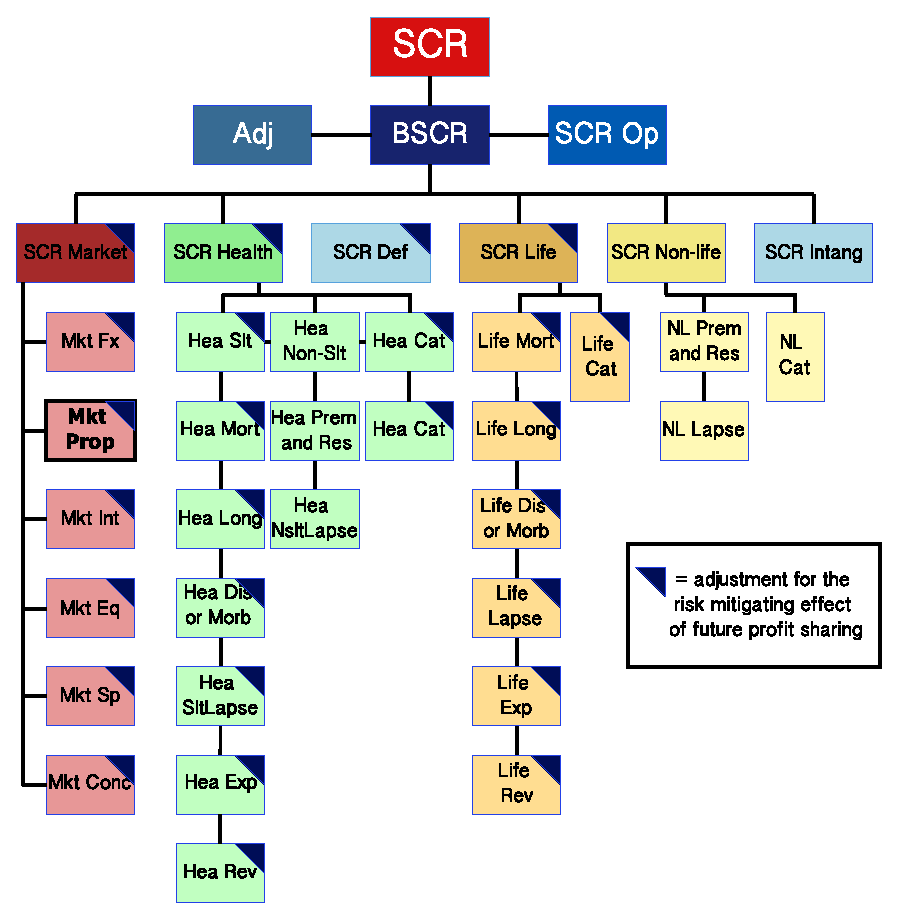
\includegraphics[scale=1]{Immagini/StrutturaSCR.eps}
\caption[Struttura del \textit{SCR}]{La struttura dei moduli e dei sottomoduli del Solvency Capital Requirement}
\label{fig:SCR}
\end{figure} 

Ogni categoria principale di rischio prevede sottorischi specifici per i settori in cui la singola compagnia opera: tali sottorischi vanno calcolati singolarmente e aggregati tramite una matrice di correlazione, che permette di considerare, nel calcolo complessivo, l'effetto di diversificazione. Un secondo effetto che il {\itshape SCR} considera, per costruzione, è quello della mitigazione del rischio derivante dal {\itshape profit sharing business}\footnote{In figura  \ref{fig:SCR} sono evidenziati i rischi per cui questo tipo di mitigazione del rischio è consentita.} e dal fondo per il differimento delle imposte.

\subsection{Il {\itshape property risk}: aspetti valutativi}
\label{subs:propertyrisk}
Una prima definizione del {\itshape property risk} viene data nella direttiva {\itshape Solvency II}\footnote{vedi art. 105, comma 5, lettera c.} che lo definisce come:
\begin{quotation} «[...] the sensitivity of the values of assets, liabilities and financial instruments to changes in the level or in the volatility of market prices of real estate».
\end{quotation}
Nelle misure di secondo livello, per lo sviluppo delle quali la commissione europea si avvale del contributo dell'EIOPA, la definizione del {\itshape property risk} cambia lievemente\footnote{La definizione nei {\itshape consulting papers} del CEIOPS diventa: «Property risk arises as a result of sensitivity of assets, liabilities and financial investments to the level or volatility of market prices of property» (\cite[p. 23]{eiopal2standardformula})}, pur mantenendo gli elementi essenziali che lo determinano.
Il {\itshape property risk} diventa quindi il livello di sensibilità che attivi, passivi e attività finanziarie hanno nei confronti del livello o della volatilità dei prezzi di mercato. L'approccio per la valutazione di tale rischio è di tipo $\Delta$-NAV: si presume uno shock di ammontare arbitrario\footnote{Questi valori sono attualmente in fase di studio e di \textit{testing} da parte delle autorità europee: nell'ultimo studio di impatto quantitativo, il quinto, l'EIOPA raccomanda di utilizzare uno shock non inferiore al 25\% \cite{eiopaqis5calibration}.} sul {\itshape net asset value} ({\itshape NAV}), ovvero la differenza fra attività e passività, sempre valutate in un'ottica {\itshape market consistent} (vedi \textit{supra} § \ref{subs:attepass}).
Possiamo sintetizzare in forma analitica il valore assunto dal requisito di solvibilità relativo al {\itshape property risk} come:

\begin{equation}
Mkt_{property} = max(\Delta NAV|_{25\%},0).
\label{for:propertyrisk}
\end{equation}
Tale formulazione poggia sull'ipotesi di uno scenario in cui il valore degli investimenti immobiliari diminuisca istantaneamente del 25\%. 
Il valore degli investimenti immobiliari è determinato dalla somma di diversi tipi di investimenti, per altro tipici dell'impresa assicurativa, esso è infatti camposo da:
\begin{itemize}
\item terreni, immobili e diritti su immobili;
\item partecipazioni (dirette o indirette) in società immobiliari che producono un reddito periodico;
\item investimenti immobiliari per l'uso proprio dell'impresa.
\end{itemize}
Per tale ragione vanno assoggettate al modello di calcolo del rischio azionario altri tipi di investimenti solo all'apparenza immobiliari, come:
\begin{itemize}
\item investimenti in società che si occupano di gestione immobiliare;
\item investimenti in società impegnate nello sivluppo di progetti immobiliari;
\item investimenti in società che hanno ricevuto prestiti da istituzioni esterne al gruppo assicurativo col fine si stimolare l'investimento in immobili.
\end{itemize}
La direttiva e le misure di secondo livello permettono, come esposto anche nella figura \ref{fig:SCR}, di ridurre il valore del fabbisogno di capitale per il {\itshape property risk} includendo nel calcolo eventuali fattori di assorbimento delle perdite.

\section{La valutazione degli immobili}
\label{sec:valimmobili}
Uno degli aspetti principali per la stima del {\itshape property risk} è il metodo di valutazione dei beni immobili detenuti dall'impresa assicurativa. 
L'approccio più diffuso in letteratura per la valutazione di un immobile prevede in prima istanza  di identificare i rendimenti attesi dal soggetto che opta per questa forma di investimento. In quest'ottica i rendimenti e il valore dell'immobile appaiono in stretta relazione fra loro, relazione che David Geltner definisce così (\cite[p. 202]{geltner}):
\begin{quotation}
«The prices investors pay for properties determine their expected returns, because the future cash flow the properties can yield is independent of the prices investors pay today for the properties».
\end{quotation}
Ciò significa che il prezzo corrisposto per l'acquisto di un immobile determina i rendimenti che l'acquirente si attende dal suo investimento, ma questi rimangono indipendenti dal prezzo iniziale.
La relazione che sussiste fra rendimenti attesi e valore dell'immobile, dato un certo prezzo di acquisto, risulta quindi essere inversa, in quanto i rendimenti futuri\footnote{nei rendimenti futuri viene incluso anche il prezzo al quale l'immobile verrà rivenduto} che l'investitore si aspetta di ricevere sono indipendenti nel tempo e sono svincolati dall'ammontare corrisposto per l'acquisto. Nello specifico i rendimenti attesi, che nella prassi corrispondono ai canoni di locazione, sono indipendenti poichè vengono determinati dall'incontro fra domanda e offerta degli immobili in locazione o, più semplicemente, dal mercato. L'indipendenza degli affitti dal prezzo corrisposto per l'acquisto dell'immobile influenza a sua volta il prezzo di vendita, poichè questo sarà, in un'ottica di continuità degli scambi, il prezzo di acquisto che il nuovo acquirente sarà disposto a pagare. Tale nuovo soggetto calcolerà il prezzo sulla base dei rendimenti attesi, ovvero delle potenziali entrate future derivanti da locazione.
\begin{figure}[htbp]
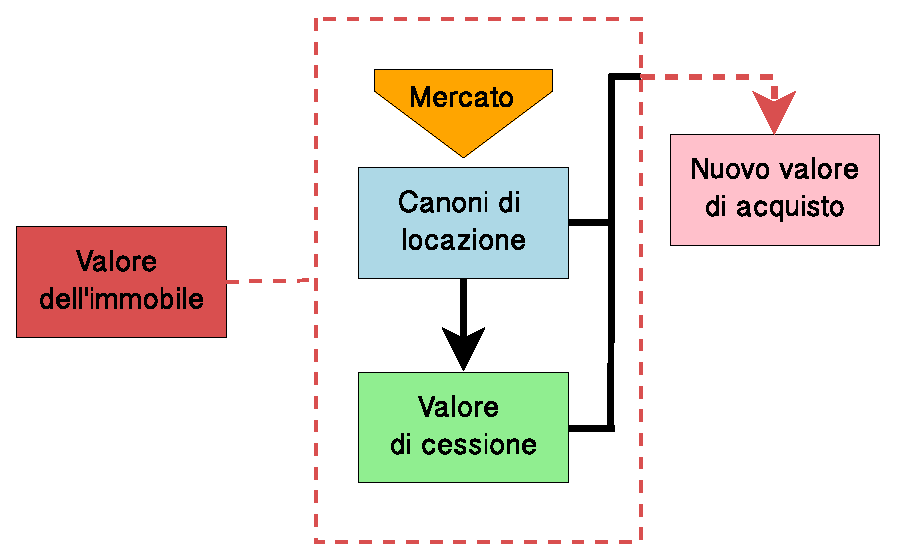
\includegraphics[scale=1]{Immagini/valoreimmobile.eps}
\caption[Sintesi della determinazione del valore di un immobile]{Il processo e le variabili che determinano il valore di un immobile}
\label{fig:valoreimmobile}
\end{figure} 

La figura \ref{fig:valoreimmobile} illustra il processo che viene compiuto ad ogni valutazione che coinvolge l'immobile di riferimento, evidenziando il ruolo svolto dal mercato nella determinzione dei canoni di locazione, variabile che assume un'importanza centrale nel metodo che si andrà ad illustrare.

\subsection{Discounted Cash Flow}
\label{subs:dcf}
Una delle procedure di valutazione più importanti nella microeconomia applicata al {\itshape real estate} è sicuramente il {\itshape multiperiod discounted cash flow} (da qui in avanti abbreviato in {\itshape DCF}). Questo sistema, utilizzato anche per lo svolgimento di questo lavoro, si sostanzia di tre momenti:
\begin{enumerate}
\item stimare i flussi di cassa attesi;
\item definire il rendimento totale che ci aspetta dall'invetimento immobiliare;
\item scontare al valore attuale i flussi di cassa al tasso di rendimento definito.
\end{enumerate}
Questi tre momenti si sostanziano analiticamente nella formula \ref{for:dcf}:
\begin{equation}
V = \frac{E_0[CF_1]}{1+E_0[r]} + \frac{E_0[CF_2]}{(1+E_0[r])^2} + \ldots + \frac{E_0[CF_{T-1}]}{(1+E_0[r])^{T-1}} + \frac{E_0[CF_T]}{(1+E_0[r])^T}.
\label{for:dcf}
\end{equation}
dove:
\begin{description}
\item $ V = $ valore attuale dell'immobile;
\item $ CF_{t} = $ flussi di cassa generati dall'immobile\footnote{nella prassi i flussi di cassa corrispondono alle cifre incassate dall'affitto dell'immobile di riferimento.} nel periodo $ t $;
\item $ E_0[r] = $ tasso medio atteso per periodo, che corrisponde al costo opportunità del capitale (da qui in poi \textit{OCC}\footnote{acronimo di {\itshape opportunity cost of capital}.}) dell'investimento immobiliare;
\item $ T = $ periodo finale dell'intera durata dell'investimento che, per convenzione, è anche il periodo in cui l'immobile verrà venduto.
\end{description}
Il valore attuale che deriva da questo sistema di calcolo si riferisce alle attese, riguardo flussi di cassa e rendimenti, del soggetto che effettua la stima. Tali attese potrebbero, in scenari come quelli di un mercato dove l'informazione non è completa e può essere asimmetrica, discostarsi dal valore effettivo a cui l'immobile potrebbe essere venduto. Se, per esempio, il risultato del calcolo secondo i \textit{DCF} fosse superiore all'effettivo prezzo di vendita, avremmo una situazione di guadagno per il venditore e perdita, in termini di costo opportunità\footnote{questo perchè il rendimento atteso del compratore sarebbe in realtà inferiore a quello utilizzato per i calcoli.}, per il compratore\footnote{il risultato sarebbe invertito qualora il valore individuato con il metodo dei \textit{DCF} fosse fosse inferiore prezzo di vendita.}.

\subsection{L'\textit{OCC} come fattore di rischio}
\label{subs:occ}
Il modello dei \textit{DCF} si basa su stime che spesso sono affidate alle capacità e alla sensibilità dell'analista; in particolare appare ragionevolmente complicato riuscire a stimare con precisione l'\textit{OCC}, che, per giunta, mutando nel tempo, dovrebbe tendere ad un incremento, rappresentativo di un aumento di rischio, per i flussi di cassa più lontani. L'\textit{OCC}, che ha la funzione di convertire un valore futuro (i flussi di cassa) in un valore corrente, è un fattore rappresentativo di due rischi distinti: da un lato il rischio insito nel variare del valore del denaro nel tempo, dall'altro quello che i flussi di cassa più distanti non si trasformino in canoni effettivamente riscossi.
Il tasso di rendimento ($ E_0[r] $ della \ref{for:dcf}, p. \pageref{for:dcf}) può essere quindi visto come somma di due componenti principali: una componente {\itshape risk-free} e una di premio di rischio (o {\itshape risk premium}). 
\begin{equation}
r = r_f + RP.
\label{for:r}
\end{equation}
La prima componente riguarda la variazione del valore del denaro nel tempo, mentre la seconda si riferisce al rischio che i flussi di cassa futuri non corrispondano ai flussi futuri reali.
Questa seconda parte di rischio è la più mutevole della somma descritta nella \ref{for:r}, poichè può essere ridimensionata in caso siano presenti dei contratti di locazione per i periodi cui il tasso di rendimento si riferisce. La presenza di un contratto permette di diminuire il rischio di un'asimmetria fra flussi attesi e flussi reali futuri, riducendo, in casi estremi, il rischio del rendimento alla sola parte {\itshape risk-free} ($ r_f $).

\subsection{L'{\itshape Interlease Discount Rate}}
\label{subs:idr}
Alla luce di quanto descritto nel paragrafo \ref{subs:occ} è necessario computare un secondo tasso di sconto da applicare a tutti i periodi successivo o al di fuori di quelli coperti da contratti di locazione: tale tasso consiste in un maggiore {\itshape risk premium} dovuto all'aumento del rischio derivante da flussi di cassa più incerti.
Questo rischio modifica sensibilmente la formula dei \textit{DCF} (\ref{for:dcf}) che possiamo riscrivere, inserendo il nuovo tasso $i$ ottenendo la \ref{for:dcfinter}.
Il nuovo tasso di sconto prende il nome di {\itshape interlease dicount rate}
\begin{equation}
V = \underbrace{\sum_{t=1}^{m} \frac{E_0[CF_1]}{1+E_0[r]}}_\textit{Periodi con contratti} + \underbrace{\underbrace{\left(\frac{1}{(1+E_0[i])^m}\right)}_\textit{Interlease DR} \cdot \underbrace{\left(\sum_{t=1}^{n-1} \frac{E_0[CF_{1}]}{(1+E_0[r])^{1}} \right)}_\textit{Periodi futuri}}_\textit{Periodi futuri privi di contratti di locazione} + \underbrace{\frac{E_0{CF_n}}{(1+E_0[i])^n}}_\textit{Valore di cessione} .
\label{for:dcfinter}
\end{equation}
dove i parametri sono i medesimi della \ref{for:dcf} e in aggiunta:
\begin{description}
\item $ i $ = {\itshape interlease discount rate};
\item $ m $ = ultimo periodo di applicazione di un tasso determinato dall'esistenza di un  contratto;
\item $ n $ = periodo finale della valutazione in cui si suppone la cessione dell'immobile.
\end{description}
Appare intuitivo constatare che l'{\itshape interlease discount rate} (da qui innanzi {\itshape IDR}) sarà, salvo casi eccezionali\footnote{un esempio in questo senso è il caso in cui si è certi di affittare l'immobile in un periodo successivo ai primi, ma a ben vedere si tratta di un numero assai limitato di casi.}, sempre maggiore dell'\textit{OCC} dei primi periodi, in quanto rappresentativo di un rischio maggiore dovuto all'incertezza di un evento futuro.

\subsection{Il {\itshape vacancy rate}}
\label{subs:vacancyrate}
Il {\itshape vacancy rate} è un fattore ampiamente usato in macroeconomia che esprime la percentuale di immobili non occupati sul totale di quelli disponibili. Questo dato, alla stregua di altri rapporti analoghi -- si pensi al tasso di disoccupazione -- assume per natura un valore diverso da zero, perchè, in termini di economicità, non è conveniente che un proprietario affitti un immobile al primo soggetto che lo richiede e, analogamente, non è conveniente per chi ricerca un immobile accettare la prima proposta. Tale non convenienza deriva dal fatto che ci sono dei costi per entrambe le parti alla stipula del contratto e dal basso costo della ricerca di offerte migliori: il tempo necessario per la ricerca di un immobile o di un conduttore genera il {\itshape vacancy rate}. Un altro motivo che giustifica l'esistenza di questo tasso è l'asimmetria nei tassi di crescita di domanda e offerta di immobili.
In generale il {\itshape vacancy rate} si attesta su un valore naturale dato dalla sua media nel lungo periodo.

Il {\itshape} vacancy rate può assume valori inferiori o superiori rispetto al suo valore naturale, e in entrambi i casi possiamo prevedere con buona approssimazione i cambiamenti nel mercato:
\begin{itemize}
\item se $vr > vr_n$, i canoni di affitto tenderanno a diminuire;
\item se $vr < vr_n$, i canoni di affitto tenderanno a crescere e potrebbe iniziare una fase espansiva dell'offerta (nuove costruzioni).
\end{itemize}

Nell'ambito del modello di seguito proposto (v. \textit{ultra} § \ref{sec:modello}), il {\itshape vacancy rate} assume una funzione analoga, ancorchè limitata ad un immobile. Come si avrà modo di analizzare nel § \ref{subs:datiinput}, il modello sviluppato utilizza dati relativi ad immobili composti da più locali (per ipotesi tutti uffici): in questo caso il {\itshape vacancy rate} indicherà la quantità di locali non affittati sul totale dei locali che compongono l'immobile.


\section{Modello proposto}
\label{sec:modello}
Il modello utilizzato nel prosieguo di questo lavoro è basato sul metodo dei \textit{DCF} (vedi \textit{supra} § \ref{subs:dcf}) ed è stato sviluppato con il \textit{software} MATLAB. Per un approfondimento sui codici del programma si rimanda all'appendice \ref{app:listatomatlab} (p. \pageref{app:listatomatlab}), mentre per i risultati dei diversi scenari si rimanda ai successivi paragrafi dove sono riportati in forma tabellare.

Data l'architettura del programma utilizzato e l'elevato numero di calcoli, è stato necessario -- e più agevole -- lavorare mediante una struttura matriciale, dove ogni variabile rappresentava una dimensione ulteriore e ogni vettore conteneva la serie di dati della variabile. Ogni matrice così costituita rappresenta un singolo immobile e il programma sviluppato usava in sequenza la matrice di ogni immobile, contenuta in un singolo input file.

\subsection{Dati in input}
\label{subs:datiinput}
Il programma sviluppato legge diversi dati di input, ma solo alcuni di essi sono fondamentali per il suo funzionamento:
\begin{itemize}
\item i flussi di cassa di ciascun periodo ($CF_i$);
\item il tasso di interesse, l'\textit{OCC} di ogni periodo ($E_0[r]$);
\item il valore stimato di vendita.
\end{itemize}
Rappresentano invece dati opzionali per il funzionameto del modello:
\begin{itemize}
\item l'{\itshape interlease discount rate};
\item il {\itshape vacancy rate}.
\end{itemize}
Un dato fondamentale, che il programma non richiede, è il numero di periodi di analisi; tale dato non è necessario in quanto il programma lo ricava da sé misurando la lunghezza del vettore dei flussi di cassa. Vale la pena ricordare che è necessario, affinchè il programma funzioni, avere vettori di uguale lunghezza.
Il cuore del programma è basato sulla formula \ref{for:dcfinter}, per tanto il valore di cessione dell'immobile è scorporato dal vettore dei flussi di cassa e si considerà come uno scalare (o vettore unitario).
Le serie storiche utilizzate per estrarre i dati appartengono a fonti diverse:
\begin{itemize}
\item per i flussi di cassa e il valore di vendita è stato utilizzato il database di {\itshape scenari immobiliari};
\item i tassi di interesse sono stati ricavati dai dati dell'{\itshape IPD} estratti dal database {\itshape Bloomberg}.
\end{itemize}
Per le analisi che hanno previsto l'utilizzo di \textit{IDR} e di {\itshape vacancy rates}:
\begin{itemize}
\item gli \textit{IDR} sono stati calcolati sulla base degli \textit{OCC} e secondo ipotesi;
\item i {\itshape vacancy rates} sono stati estratti dal database della Jonas Lang LaSalle.
\end{itemize}

I dati utilizzati per i calcoli sono tutti relativi ad immobili (composti ciascuno da un numero di uffici compreso fra le 20 e le 30 unità) selezionati nelle aree del centro e immediatamente limitrofe di cinque città italiane\footnote{i dati si riferiscono alle città di Milano, Roma, Torino, Bologna e Padova, per ulteriori specificazioni si rimanda all'Appendice \ref{app:datiimmobili}.}. La metratura media di ogni ufficio varia in funzione della città, come esposto nella tabella \ref{tab:metrature}.
\begin{table}[htbp]
\begin{center} \begin{tabular}{|c|c|c|}
\hline
{\bfseries Città} & {\bfseries Metratura media} & {\bfseries Uffici per immobile} \\
\hline
Milano & 200 & 20 \\
\hline
Roma & 100 & 20 \\
\hline
Torino & 90 & 25 \\
\hline
Bologna & 90 & 25 \\
\hline
Padova & 85 & 30\\
\hline
\end{tabular} \end{center}
\caption{Numero di uffici e metratura media distinti per città}
\label{tab:metrature}
\end{table}
Per una maggiore comparabilità dei risultati si è scelto di lavorare con i dati medi riportati nella tabella \ref{tab:metriufficimedi}:
\begin{table}[htbp]
\begin{center} \begin{tabular}{|c|c|c|}
\hline
{\bfseries Città} & {\bfseries Metratura media} & {\bfseries Uffici per immobile} \\
\hline
Tutte & 113 $\approx$ 115 & 24 $\approx$ 25 \\
\hline
\end{tabular} \end{center}
\caption{Valori medi di metratura e uffici}
\label{tab:metriufficimedi}
\end{table}
Tali ipotesi non hanno impatti rilevanti sui risultati finali e consentono una migliore percezione dei dati elaborati, in quanto un prezzo espresso al metro quadro o al metro quadro per anno è meno agevole da leggere più difficile da confrontare rispetto al valore dell'intero immobile.

\subsection{Risultati per lo scenario base}
\label{subs:risultatiscenbase}
Lo scenario basilare prevede l'applicazione del modello ai soli dati fondamentali descritti al paragrafo \ref{subs:datiinput}, vale a dire flussi di cassa, valore di cessione e rendimenti. In questa prima fase si suppone che gli immobili siano sempre affittati ({\itshape vacancy rate} nullo) e che tutti i contratti futuri siano già stati stipulati {\itshape IDR nullo}.
Nella tabella \ref{tab:dcfmirotobopd} sono riportati i risultati per singolo immobile raggruppati per città..

% Tabelle DCF Milano, Roma, Torino, Bologna, Padova
\begin{table}[htbp]
\begin{center} 
\begin{tabular}[c]{|l||c|}
\hline
{\bfseries Milano} & {\bfseries \textit{DCF}} \\
\hline \hline
Imm. 1 & 16.205.885 \\
\hline
Imm. 2 & 24.732.349 \\
\hline
Imm. 3 & 31.542.120 \\
\hline
Imm. 4 & 26.129.468 \\
\hline
\end{tabular}
\hspace{5mm}
\begin{tabular}[c]{|l||c|}
\hline
{\bfseries Roma} & {\bfseries \textit{DCF}} \\
\hline \hline
Imm. 1 & 38.120.230 \\
\hline
Imm. 2 & 26.640.321 \\
\hline
Imm. 3 & 24.548.218 \\
\hline
Imm. 4 & 22.257.105 \\ 
\hline
\end{tabular}
\hspace{5mm}
\vspace{1cm}
\begin{tabular}[c]{|l||c|}
\hline
{\bfseries Torino} & {\bfseries \textit{DCF}} \\
\hline \hline
Imm. 1 & 9.220.290 \\
\hline
Imm. 2 & 16.453.004 \\
\hline
Imm. 3 & 24.548.218 \\
\hline
Imm. 4 & 9.172.760 \\
\hline
\end{tabular} 
\hspace{5mm}
\begin{tabular}[c]{|l||c|}
\hline
{\bfseries Bologna} & {\bfseries \textit{DCF}} \\
\hline \hline
Imm. 1 & 15.439.025 \\
\hline
Imm. 2 & 13.411.647 \\
\hline
Imm. 3 & 15.168.141 \\
\hline
Imm. 4 & 14.600.870 \\
\hline
\end{tabular} 
\hspace{5mm}
\begin{tabular}[c]{|l||c|}
\hline
{\bfseries Padova} & {\bfseries \textit{DCF}} \\
\hline \hline
Imm. 1 & 13.124.147 \\
\hline
Imm. 2 & 13.946.266 \\
\hline
Imm. 3 & 12.469.543 \\
\hline
Imm. 4 & 13.140.184 \\
\hline
\end{tabular} 
\caption[DCF per gli immobili scelti]{DCF per gli immobili siti a Milano, Roma, Torino, Bologna e Padova}
\label{tab:dcfmirotobopd}
\end{center}
\end{table}

Si ricorda che i risultati sono calcolati sulla base delle ipotesi di metratura media e composizione degli immobili riportate al § \ref{subs:datiinput} e che i dati relativi ai canoni e all'ubicazione dei singoli immobili sono riportati in Appendice \ref{app:datiimmobili}.
L'\textit{OCC} utilizzato è il tasso medio dell'indice ISI di settore\footnote{nello specifico l'{\itshape Italy ISI Property Offices} reperibile su \textit{Bloomberg} con il \textit{Ticker} ITHPO.} elaborato da Scenari Immobiliari SpA, relativo agli ultimi dieci anni. I valori si intendono espressi in euro.
Di seguito, nella tabella \ref{tab:dcfbasedescrittive}, si evidenziano le principali statistiche descrittie sui dati prodotti dal modello aggregati per città.

% Tabella statistiche descrittive DCF Scenario Base
\begin{table}[htbp]
\label{tab:dcfbasedescrittive}
\begin{center}
\begin{tabular}[c]{|l||*{5}{c|}}
\hline
{\bfseries Città} & {\bfseries Obs} & {\bfseries Media DCF} & {\bfseries Std. Dev.} DCF & {\bfseries Min} & {\bfseries Max} \\
\hline \hline
Milano & 4 & 24.652.456 & 6350852,41 & 16.205.885 & 31.542.120 \\
\hline
Roma & 4 & 27.891.469 & 7050208,22 & 22.257.105,00 & 38.120.230 \\
\hline
Torino & 4 & 14.848.568 & 7315502,60 & 9.172.760 & 24.548.218 \\
\hline
Bologna & 4 & 14.654.921 & 899419,37 & 13.411.647 & 15.439.025 \\
\hline
Padova & 4 & 13.170.035 & 604488,87 & 12.469.543 & 13.946.266 \\
\hline
{\itshape Totale} & 20 & 19.043.490 & 7808886,69 & 9.172.760 & 38.120.230 \\
\hline
\end{tabular}
\caption{Principali statistiche descrittive sui dati prodotti dal modello}
\end{center}
\end{table}

\chapter{Analisi di sensitività}
\label{chap:ansens}
Sulla base del modello descritto al capitolo precedente sono state sviluppate diverse analisi di sensitività rispetto alle variabili che determinano il valore del modello proposto. Tali simulazioni, univariate, realizzate tramite il programma di calcolo \textit{MATLAB}\footnote{I codici del programma creato sono riportati nell'appendice \ref{app:listatomatlab}.}, si basano sulla simulazione di variazioni (o \textit{shock}) sulle variabili ritenute di maggior impatto sul valore finale. Nei paragrafi che seguono sono riportati in sintesi i principali risultati, disponibili anche in valore assoluto (espressi in euro) nell'appendice \ref{app:risultati}.

\section{La sensitività dei flussi di cassa}
\label{sec:simvcf}
L'analisi della dipendenza del modello dei \textit{DCF} dai {\itshape cash flows}, ovvero dal livello delle entrate attese, si sviluppa in due direzioni: la prima simulazione prende in considerazione una variazione limitata ai soli affitti, la seconda  ipotizza che la variazione coinvolga anche l'ammontare finale a cui si stima di vendere l'immobile.
Ad una prima impressione la prima simulazione può sembrare superflua o almeno parzialmente distante dalla realtà del mercato immobiliare, tuttavia lo scenario simulato non è improbabile, ancorchè raro. Un esempio in tal senso può essere l'ipotesi di una bolla speculativa che all'ultimo periodo faccia rivalutare l'immobile, o meglio rimuova il fattore di shock. Un altro caso che trova applicazione nella prima simulazione è quello descritto dalla teoria del cosiddetto {\itshape greater fool} (\cite[p. 203]{geltner}), teoria secondo la quale un investimento frutto di una valutazione errata potrà essere \textit{ceduto} ad un più grande \textit{fool} presente sul mercato.
Le simulazioni svolte ipotizzano shock progressivi in base 5\% con una magnitudo del 25\% del valore, sia per gli scenari positivi che per quelli negativi. La misura della magnitudo deriva dalle specifiche tecniche riportare per il {\itshape property risk} all'interno dei documenti tecnici dell'EIOPA in merito al {\itshape QIS 5} (\cite[p. 174]{qistechnical}).

\subsection{Prima ipotesi: shock solo sugli affitti}
\label{subs:vcf1}
I risultati della simulazione sono riportati in sintesi nella tabella \ref{tab:varvcfsintesi}: le statistiche descrittive si riferiscono all'insieme degli immobili presi in considerazione e le percentuali si riferiscono al valore medio di tutti i rapporti fra ciascun \textit{DCF} post-shock e il rispettivo valore ottenuto nello scenario base (ovvero con shock pari a 0\%).
% Tabelle VCF Sintesi in Percentuale
\begin{table}[htbp]
\begin{center}
\begin{tabular}[c]{|c||*{4}{c|}}
\hline
$\Delta$ CF & Media & Passo & Dev Std. & Mediana \\
\hline \hline
-25\% & -8.05\% & -1.61\% & 0.003674522 & -8.02\% \\ \hline
-20\% & -6.44\% & -1.61\% & 0.002939616 & -6.41\% \\ \hline
-15\% & -4.83\% & -1.61\% & 0.002204711 & -4.81\% \\ \hline
-10\% & -3.22\% & -1.61\% & 0.001469812 & -3.21\% \\ \hline
-5\% & -1.61\% & -1.61\% & 0.000734898 & -1.60\% \\ \hline
SB & 0.00\% & 0.00\% & 0.00 & 0.00\% \\ \hline
5\% & 1.61\% & 1.61\% & 0.000734907 & 1.60\% \\ \hline
10\% & 3.22\% & 1.61\% & 0.001469815 & 3.21\% \\ \hline
15\% & 4.83\% & 1.61\% & 0.002204723 & 4.81\% \\ \hline
20\% & 6.44\% & 1.61\% & 0.002939625 & 6.41\% \\ \hline
25\% & 8.05\% & 1.61\% & 0.003674534 & 8.02\% \\ \hline
\end{tabular}
\caption[Media risultati di $\Delta$ CF]{La media dei risultati delle simulazioni sulla variazione dei {\itshape cash flows} per gli immobili esaminati}.
\label{tab:varvcfsintesi}
\end{center}
\end{table}


Il primo dato che possiamo osservare è che l'andamento del \textit{DCF} a seguito di uno shock è perfettamente simmetrico e lineare, con passo di $0.0161$. La simmetria si ha in quanto il valore assunto dalla media dei {\itshape discounted cash flows} cambia il segno in base a quello dello shock che è stato simulato, ma resta identico in valore assoluto. Il coefficiente angolare della retta che descrive l'andamento della media dei \textit{DCF} post-shock è di circa $0.0322$. 
La linearità dei \textit{DCF} in relazione ai \textit{CF} è una caratteristica fisiologica del modello  ed è riscontrabile nel calcolo del valore di tutti gli immobili in esame (si vedano in merito le tabelle \ref{tab:rvcf1-1} e \ref{tab:rvcf1-2} allegate nell'appendice \ref{app:risultati}).

I risultati ottenuti sono descritti anche graficamente nella Figura \ref{graf:varvcf}.
Il grafico a barre descrive la relazione fra valore medio dei \textit{DCF} e shock simulati e la linearità di tale relazione è descritta dalla diagonale tratteggiata.
% Grafico Variazione DCF vs shock CF
\begin{figure}[htbp]
\begin{center}
{\includegraphics[scale=0.40]{Grafici/Terzo/varvcf.eps}}
\caption[Variazione media \% dei \textit{DCF} vs $\Delta$ di \textit{CF}]{Variazione percentuale media dei \textit{DCF} agli shock simulati}
\label{graf:varvcf}
\end{center}
\end{figure}

\subsection{Seconda ipotesi: shock su affitti e valore finale}
\label{subs:vcf2}
Lo scenario più probabile in caso di uno shock sulle entrate che un immobile produce è che questo coinvolga sia i canoni di locazione che l'eventuale futuro valore di cessione: in questo paragrafo si analizzano i risultati della simulazione di uno shock, quantitativamente identico al paragrafo precedente (\ref{subs:vcf1}), che coinvolge entrambe queste grandezze.
Come prevedibile, alla luce anche dei risultati della simulazione precedente, il \textit{DCF} dimostra di dipendere, per costruzione, in maniera lineare dagli importi che costituiscono i flussi di cassa. La simulazione in analisi dimostra infatti che, se lo shock impatta identicamente su canoni d'affitto e valore di cessione, il \textit{DCF} si contrae o espande del medesimo valore. La direzione del cambiamento di valore è correlata positivamente al segno dello shock. Nella tabella \ref{tab:varvcf2} sono riportati i risultati, mentre la Figura \ref{graf:varvcf2} descrive la relazione lineare unitaria fra shock e variazione della media dei \textit{DCF}. 
% Tabelle VCF Sintesi in Percentuale
\begin{table}[htbp]
\begin{center}
\begin{tabular}[c]{|c||*{4}{c|}}
\hline
$\Delta$ CF & Media & Passo & Dev Std. & Mediana \\
\hline \hline
-25\% & -25\% & -5.00\% & $\approx$ 0.00 & -25\% \\ \hline
-20\% & -20\% & -5.00\% & $\approx$ 0.00 & -20\% \\ \hline
-15\% & -15\% & -5.00\% & $\approx$ 0.00 & -15\% \\ \hline
-10\% & -10\% & -5.00\% & $\approx$ 0.00 & -10\% \\ \hline
-5\% & -5\% & -5.00\% & $\approx$ 0.00 & -5\% \\ \hline
SB & 0.00\% & 0.00\% & 0.00 & 0.00\% \\ \hline
5\% & 5\% & 5.00\% & $\approx$ 0.00 & 5\% \\ \hline
10\% & 10\% & 5.00\% & $\approx$ 0.00 & 10\% \\ \hline
15\% & 15\% & 5.00\% & $\approx$ 0.00 & 15\% \\ \hline
20\% & 20\% & 5.00\% & $\approx$ 0.00 & 20\% \\ \hline
25\% & 25\% & 5.00\% & $\approx$ 0.00 & 25\% \\ \hline
\end{tabular}
\caption[Media risultati di $\Delta$ CF e valore di cessione]{La media dei risultati delle simulazioni sulla variazione dei {\itshape cash flows} e del valore di cessione per gli immobili esaminati.}.
\label{tab:varvcf2}
\end{center}
\end{table}

% Grafico Variazione DCF vs shock CF
\begin{figure}[htbp]
\begin{center}
{\includegraphics[scale=0.40]{Grafici/Terzo/varvcf2.eps}}
\caption[Variazione media \% dei \textit{DCF} vs $\Delta$ di \textit{CF} e valore di cessione]{Variazione percentuale media dei \textit{DCF} agli shock simulati sui \textit{CF} e sul valore di cessoine}
\label{graf:varvcf2}
\end{center}
\end{figure}

\section{Analisi dell'{\itshape interlease discount rate}}
\label{sec:simvidr}
L'{\itshape interlease discount rate} è un fattore di rischio del modello \textit{DCF} che dipende in larga misura dalla sensibilità del soggetto che compie la valutazione di un immobile. Se si osserva più da vicino la prassi del mercato immobilare si può notare che l'\textit{IDR} non viene quasi mai utilizzato, a vantaggio di un unico \textit{OCC} comprensivo anche di questa parte di rischio. Tale approccio risulta sicuramente più pratico, ma, a parità di approssimazione della stima, è meno preciso. Per questa ragione l'analisi qui svolta analizza separatamente i due tassi (per le analisi sul \textit{OCC} si veda il paragrafo \ref{sec:simvocc}), che hanno per altro una natura diversa. L'\textit{IDR} infatti mira a quantificare l'incertezza di uno o più flussi di cassa futuri, mentre l'\textit{OCC} rappresenta il tasso che si sarebbe potuto ottenere investendo diversamente il flusso di cassa.
L'ipotesi alla base dell'analisi svolta è che i primi quattro flussi di cassa siano certi, per tanto calcolati sulla base del solo \textit{OCC}, e che i successivi sei flussi siano incerti\footnote{Si ipotizza quindi che solo i primi quattro canoni di locazione siano contrattualizzati.}, quindi scontati per l'\textit{OCC} e per l'\textit{IDR}, che sconta anche il valore di cessione che viene incassato al decimo ed ultimo periodo.
Sulla scorta di questa semplice ipotesi si è svolta l'analisi di scenario che, partendo dallo scenario base, per coerenza, è stata svolta in un'unica direzione, quella positiva, in quanto per definizione l'\textit{IDR} può essere al minimo pari all'\textit{OCC}. Gli scenari ipotizzati consistono in una serie di aumenti di 100bp (1\%) a partire dal costo-opportunità del capitale che, nello scenario base è pari a 4.875\%, fino ad un {\itshape worst case scenario} del 12.875\% che rappresenta il caso limite in cui al costo-opportunità del capitale venga aggiunto un premio per il rischio dell'8\%. La scelta del valore estremo di questa magnitudo va fatta risalire all'interesse massimo sostenibile dal Paese di riferimento -- l'Italia nel caso in esame -- sui propri titoli di stato con la scadenza più simile alla struttura dell'operazione che stiamo valutando. Data questa premessa, un tal valore soglia è stato stimato da Banca d'Italia nella misura dell'8\% (\cite[p. 59]{rapportobdistabilita}) per i BTP decennali.

La tabella \ref{tab:varidrsintesi} riporta le principali statistiche descrittive ricavate dai risultati ottenuti: è di facile identificazione il comportamento della media dei \textit{DCF} che ha un andamento strettamente decrescente all'aumentare dello shock indotto sull'\textit{IDR}: ciò implica che all'aumentare dell'\textit{IDR} il valore dei \textit{DCF} si ridurrà, ma in misura sempre minore. Questo tipo di andamento è descritto graficamente dalla Figura \ref{graf:varidr}, elaborata sulla base dei risultati ottenuti nella simulazione.
% Tabelle IDR Sintesi in Percentuale
\begin{table}[htbp]
\begin{center}
\begin{tabular}[c]{|c||*{4}{c|}}
\hline
IDR & Media & Passo & Dev Std. & Mediana \\
\hline \hline
5.875\% & -30.2\% &  n.d. & 0.00583877 & -30.2\% \\ \hline
6.875\% & -34.2\% & -4.1\% & 0.00628121 & -34.3\% \\ \hline
7.875\% & -37.9\% & -3.7\% & 0.00666624 & -38.0\% \\ \hline
8.875\% & -41.3\% & -3.4\% & 0.00700058 & -41.3\% \\ \hline
9.875\% & -44.4\% & -3.1\% & 0.00729012 & -44.4\% \\ \hline
10.875\% & -47.2\% & -2.8\% & 0.00754009 & -47.2\% \\ \hline
11.875\% & -49.7\% & -2.6\% & 0.00775511 & -49.8\% \\ \hline
12.875\% & -52.1\% & -2.4\% & 0.00793922 & -52.1\% \\ \hline
\end{tabular}
\caption[Media risultati di un $\Delta^{+}$ IDR]{La media dei risultati delle simulazioni sull'aumento degli {\itshape IDR} per gli immobili esaminati.}
\label{tab:varidrsintesi}
\end{center}
\end{table}

% Grafico Variazione DCF vs shock IDR
\begin{figure}[htbp]
\begin{center}
{\includegraphics[scale=0.40]{Grafici/Terzo/varidr.eps}}
\caption[Variazione media \% dei \textit{DCF} vs $\Delta$ \textit{IDR}]{Variazione percentuale media dei \textit{DCF} agli shock simulati sull'\textit{IDR}}
\label{graf:varidr}
\end{center}
\end{figure}

\section{Simulazioni sul \textit{vacancy rate}}
Il {\itshape vacancy rate} è una variabile che influisce sulla {\itshape quantità di immobile} disponibili; nel caso in esame influisce sulla quantità di uffici disponibili all'interno del singolo immobile, per ipotesi stabilità in 25 unità. Il {\itshape vacancy rate} ha quindi l'effetto di ridimensionare l'ammontare dei flussi di cassa disponibili come una normale variazione dei flussi di cassa, la cui analisi è già stata svolta (in merito si veda il § \ref{sec:simvcf}).
La magnitudo degli shock è dettata dai {\itshape vacancy rate} stimati dall'\textit{IPD} che tuttavia, pur essendo l'istituzione di riferimento a livello europeo, non forniscono serie storiche per quattro delle cinque città analizzate e, per la restante (Milano), ne forniscono una poco profonda. Sulla base di ciò è stata scelta come base di partenza il 5\%\footnote{Tale dato si riferisce al primo trimestre del 2004.} che rappresenta una soglia prudenziale al di sotto del minimo rilevato nella serie storica disponibile, e come massimo il valore raggiunto da una serie  storica più profonda analoga a quella di Milano. Il dato massimo così scelto, il 12\%, è confermato anche da molti analisti di settore\footnote{Fra i vari: Scenari Immobiliari, BNP Paribas RE, CBRE.} come il valore estremo raggiungibile nei recenti anni di recessione (\cite{ilsolevacancy}, \cite[p. 3]{cbrevacancy}).
% Tabelle IDR Sintesi in Percentuale
\begin{table}[htbp]
\begin{center}
\begin{tabular}[c]{|c||*{4}{c|}}
\hline
VR & Media & Passo & Dev Std. & Mediana \\
\hline \hline
SB & 0.00\% & -1.58\% & 0.00 & 0.00\% \\ \hline
5\% & -1.58\% & -0.32\% & 0.000703832 & -1.60\% \\ \hline
6\% & -1.93\% & -0.32\% & 0.000844608 & -1.92\% \\ \hline
7\% & -2.25\% & -0.32\% & 0.000985368 & -2.25\% \\ \hline
8\% & -2.57\% & -0.32\% & 0.001126142 & -2.57\% \\ \hline
9\% & -2.89\% & -0.32\% & 0.001266908 & -2.89\% \\ \hline
10\% & -3.21\% & -0.32\% & 0.001407681 & -3.21\% \\ \hline
11\% & -3.54\% & -0.32\% & 0.001548448 & -3.53\% \\ \hline
12\% & -3.86\% & -0.32\% & 0.001689223 & -3.85\% \\ \hline
\end{tabular}
\caption[Media risultati di un $\Delta^{+}$ {\itshape vacancy rate}]{La media dei risultati delle simulazioni sulla variazione del {\itshape vacancy rate} per gli immobili esaminati.}
\label{tab:varvr}
\end{center}
\end{table}

\begin{figure}[htbp]
\begin{center}
{\includegraphics[scale=0.40]{Grafici/Terzo/varvr.eps}}
\caption[Variazione media \% dei \textit{DCF} vs $\Delta$ del {\itshape vacancy rate}]{Variazione percentuale media dei \textit{DCF} agli shock simulati sul {\itshape vacancy rate}}
\label{graf:varvr}
\end{center}
\end{figure}

Nella tabella \ref{tab:varvr} sono riportate le statistiche descrittive dei risultati dalle quali si può notare che la relazione fra {\itshape vacancy rate} e \textit{DCF} è lineare, così come nell'analisi dei flussi di cassa (si veda il § \ref{sec:simvcf}). Il grafico riportato in figura \ref{graf:varvr} descrive questo andamento per gli shock simulati sulla variabile.

\section{Simulazioni sull'\textit{OCC}}
\label{sec:simvocc}
Un altro \textit{driver} su cui si è svolta l'analisi di scenario è il costo-opportunità del capitale. Per questa variabile valgono alcune considerazioni svolte al paragrafo \ref{sec:simvidr}, la principale è che la scelta del tasso da applicare dipende in buona parte dalla capacità e dalla sensibilità di chi compie la valutazione. Il tasso utilizzato nello scenario base, come già descritto al § \ref{subs:risultatiscenbase}, è il tasso medio del segmento uffici dell'indice ISI. Per questa analisi di sensitività dell'\textit{OCC} è stato utilizzata una struttura dei tassi semplificata -- la medesima dello scenario base -- dove il tasso medio definito dall'ISI viene applicato a tutti i periodi: si presuppone quindi che l'immobile che si sta valutando sia, per i dieci anni in esame, sempre affittato. Nel prosieguo di questo lavoro è riportata anche un'analisi su una struttura dei tassi differente da quella semplificata qui proposta (in merito si rimanda al § \ref{subs:simvstr}).
Per la magnitudo degli shock simulati sulla variabile valgono le medesime considerazioni fatte per l'\textit{IDR} (v. \textit{supra} § \ref{sec:simvidr}), con, in aggiunta, degli scenari di diminuzione dell'\textit{OCC} progressivi di 100bp fino ad un minimo di 1.875\%.

La tabella \ref{tab:varoccsintesi} riporta le principali statistiche descrittive per scenario, ricavate dai risultati ottenuti (disponibili in valore assoluto espresso in euro nell'appendice \ref{app:risultati}, tabelle \ref{tab:rocc1} e \ref{tab:rocc2}). Anche nel caso in esame l'andamento del valore del \textit{DCF} è decrescente all'aumento dell'\textit{OCC}.

% Tabelle IDR Sintesi in Percentuale
\begin{table}[htbp]
\begin{center}
\begin{tabular}[c]{|c||*{4}{c|}}
\hline
OCC & Media & Passo & Dev Std. & Mediana \\
\hline \hline
1.875\% & 5.27\% &  1.89 & 0.00240804 & 5.25\% \\ \hline
2.875\% & 3.38\% &  1.75 & 0.00154391 & 3.37\% \\ \hline
3.875\% & 1.63\% &  1.63 & 0.00074312 & 1.62\% \\ \hline
4.875\% & 0\% &  n.d. & 0.00 & 0\% \\ \hline
5.875\% & -1.51\% &  -1.51 & 0.00069046 & -1.51\% \\ \hline
6.875\% & -2.92\% & -1.41 & 0.00133283 & -2.91\% \\ \hline
7.875\% & -4.23\% & -1.31 & 0.00193118 & -4.21\% \\ \hline
8.875\% & -5.45\% & -1.22 & 0.00248922 & -5.43\% \\ \hline
9.875\% & -6.59\% & -1.14 & 0.0030103 & -6.57\% \\ \hline
10.875\% & -7.66\% & -1.07 & 0.00349743 & -7.63\% \\ \hline
11.875\% & -8.66\% & -1.00 & 0.00395333 & -8.63\% \\ \hline
\end{tabular}
\caption[Media risultati di $\Delta$ \textit{OCC}]{La media dei risultati delle simulazioni sull'aumento dell'{\itshape OCC} per gli immobili esaminati.}
\label{tab:varoccsintesi}
\end{center}
\end{table}

% Grafico Variazione DCF vs shock OCC
\begin{figure}[htbp]
\begin{center}
{\includegraphics[scale=0.40]{Grafici/Terzo/varocc.eps}}
\caption[Variazione media \% dei \textit{DCF} vs $\Delta$ \textit{OCC}]{Variazione percentuale media dei \textit{DCF} agli shock simulati sull'\textit{OCC}}
\label{graf:varocc}
\end{center}
\end{figure}

La figura \ref{graf:varocc} descrive tale decremento, marginalmente sempre minore all'aumentare del tasso.


\subsection{Simulazioni sulla struttura dei tassi}
\label{subs:simvstr}
Un secondo tipo di analisi sull'\textit{OCC} può essere svolto ipotizzando una struttura dei tassi variabile nel tempo. In questo caso il numero di scenari ipotizzabili diventa infinito, ma è possibile identificare alcuni casi di elevato interesse pratico.

Nella continuazione dell'analisi sono stati scelti cinque scenari differenti:
\begin{enumerate}
\item un aumento annuale progressivo dell'\textit{OCC} dello 0.5\%  a partire dal tasso medio dello scenario base (4.875\%);
\item una diminuzione progressiva dello 0.5\% partendo dal 9.375\% (vale a dire l'inverso del primo scenario);
\item l'utilizzo dei tassi annuali medi degli ultimi dieci anni calcolati dall'\textit{IPD} per l'Italia;
\item uno scenario con minimi al primo e all'ultimo periodo e massimo nel periodo centrale;
\item uno scenario con massimi al primo e all'ultimo periodo e minimo nel periodo centrale.
\end{enumerate}
I risultati -- espressi in euro -- sono riportati nelle tabelle \ref{tab:rstr1} e \ref{tab:rstr2} nell'appendice \ref{app:risultati} e descritti graficamente nella figura \ref{graf:varstr}: per gli scenari in legenda è stato mantenuto l'ordine dell'elenco appena descritto. Il grafico esprime i valori, ciascuno contraddistinto da simboli, degli immobili, ordinati sull'asse delle ascisse, in ciascuno dei cinque scenari descritti. La linea azzurra descrive  un'interpolazione fra questi valori e facilita la rappresentazione dei rapporti di forza degli immobili all'interno del portafoglio immobiliare costruito. Per esemplificare, si può notare che il quinto immobile è quello con il maggior valore oppure che gli immobili dal sedicesimo al ventesimo (quelli cioè ubicati a Padova) hanno un valore omogeno fra loro, ma inferiore ai primi quattro (quelli ubicati a Milano) o alla quartina centrale (gli immobili ubicati a Torino).
\begin{sidewaysfigure}[htbp]
\begin{center}
{\includegraphics[scale=0.70]{Grafici/Terzo/varstr.eps}}
\caption[Confronto degli scenari di struttura dell'\textit{OCC}]{Confronto del \textit{DCF} (in \EURtm) degli immobili con cinque strutture di tassi differenti}
\label{graf:varstr}
\end{center}
\end{sidewaysfigure}

\clearpage

\section{Conclusioni}
Nel corso dell'analisi di sensitività descritta all'interno di questo capitolo si è potuto constatare che i fattori analizzati hanno un'incisività diversa sul valore finale del \textit{DCF}. 

I fattori che influiscono sull'ammontare dei flussi di cassa\footnote{Valore degli affitti, valore di cessione dell'immobile e {\itshape vacancy rate}.}, e cioè sul numeratore della formula  \ref{for:dcfinter}, incidono linearmente sull'ammontare finale del \textit{DCF} e, nello scenario più drastico, quando vi è collinearità fra shock sugli affitti e shock sul valore di cessione (§  \ref{subs:vcf1}), la riduzione percentuale del valore del \textit{DCF} è identica a quella della riduzione occorsa alla variabile.

Diversamente, la variazione dei fattori\footnote{\textit{OCC}, \textit{IDR} e, per certi tipi di analisi la struttura dei tassi} che influiscono sul denominatore della formula \ref{for:dcfinter} non ha effetti lineari sul valore dei {\itshape discount cash flows}. In questo caso ad un aumento di un fattore corrisponde una diminuzione del \textit{DCF} di portata diversa a seconda del fattore preso in analisi.
Nel caso di una simulazione univariata sull'\textit{OCC} (§ \ref{sec:simvocc}) il decremento del \textit{DCF} ha un ordine di grandezza in linea con quello dello shock ipotizzato sulla variabile, come illustrato nella tabella \ref{tab:varoccsintesi}, mentre altrettanto non avviene per un'analoga simulazione condotta sull'\textit{IDR} (§ \ref{sec:simvidr}): in questo caso infatti l'ordine di grandezza della variazione del \textit{DCF} è di circa cinque volte superiore rispetto a quello dello shock. Questo effetto è intrinseco alla costruzione del modello analizzato, che ipotizza di scontare a tassi più rischiosi, e quindi maggiori, i flussi più lontani che includono anche il valore di cessione. Possiamo dunque affermare che questa quantità è il motivo principale per cui il valore indicato dal modello \textit{DCF}\footnote{Nella versione che esplicita l'\textit{IDR} descritta alla formula \ref{for:dcfinter}} risulta così fortemente ridimensionato.

In conclusione possiamo affermare che, in un'analisi univariata, il modello dei \textit{DCF} risulta più sensibile alle variazioni dell'\textit{IDR} rispetto all'\textit{OCC}, pur non tralasciando l'importanza della scelta di una struttura dei tassi coerente con il mercato di riferimento dell'immobile -- o del portafoglio di immobili -- che si valuta. Va inoltre aggiunto che, a seconda della strategia scelta per la valutazione\footnote{Questa dipenderà dagli obiettivi e dalle eventuali norme che regolano la valutazione} e della portata degli shock, possono influenzare il valore del \textit{DCF}, in maniera apprezzabile, anche il {\itshape vacancy rate} e le altre variabili di variazione dei {\itshape cash flows}.
\chapter{Analisi di scenario multivariata}
Dopo l'analisi di sensibilità svolta sui singoli fattori che caratterizzano il modello dei {\itshape discounted cash flows} si rende necessaria un'analisi che identifichi le dipendenze fra le diverse variabili in gioco nel principale modello valutativo del settore del {\itshape real estate}. Questa analisi rappresenta quindi una continuazione, su un livello diverso, di quella condotta al capitolo \ref{chap:ansens} e, al contempo, uno strumento veicolare al raggiungimento di un risultato confrontabile e utilizzabile per valutare le disposizioni di {\itshape Solvency II} riguardo al {\itshape property risk}.

\section{L'interdipendenza delle variabili}
È stato evidenziato nel capitolo precedente che modello dei \textit{DCF} dipende da diverse variabili: la prima categoria raccoglie tutte quelle che influiscono sui livelli degli affitti ({\itshape rent levels}), come il {\itshape vacancy rate}, mentre la seconda comprende le variabili utilizzate per scontare i flussi di cassa.
Nell'analisi che si intende svolgere in questo capitolo occorre, in prima istanza, analizzare qualitativamente la dipendenza di queste variabili dal mercato {\itshape real estate}, dipendente dalla domanda e dall'offerta di immobili e, ad un livello superiore, da altri mercati e, più in generale, dalla congintura economia.
In questo senso risulta utile descrivere i fenomeni che possono coinvolgere le variabili descritte.

Il {\itshape vacancy rate}\footnote{Relativamente al mercato di riferimento del campione analizzato in questo lavoro, ovvero gli uffici} dipende dalla quantità di edifici, totali e disponibili, dai livelli occupazionali dei settori coinvolti e dal livello degli affitti. Come già accennato al § \ref{subs:vacancyrate}, il {\itshape vacancy rate} è un indicatore di equilibrio fra domanda e offerta piuttosto che un indicatore di una di queste due misure. Semplificando possiamo dire che è una buona sintesi del rapporto delle misure da cui dipende.
Risulta quindi ragionevole dire che, in un mercato perfetto, se la domanda di immobili -- uffici in affitto, in questo caso -- aumenta, aumenterà di una certa quantità anche il livelli degli affitti.
Il driver principale che influenza la domanda di uffici è il livello occupazionale nel settore finanziario, principalmente bancario, assicurativo e immobiliare, e nel settore sei servizi legali e professionali \cite[p. 112]{geltner}: risulta lapalissiano considerare che un maggior numero di lavoratori richiederà un maggiore spazio lavorativo.
A ciò va aggiunta la correlazione negativa fra il livello degli affitti e il {\itshape vacancy rate}, che in questo scenario diminuirà.  
Analoghe e opposte considerazioni possono essere svolte considerando aumenti o diminuzioni nel livello dell'offerta degli immobili, che dipende in gran parte dalla quantità di nuove costruzioni e quindi dalle concessioni amministrative\footnote{Occorre quindi verificare eventuali vincoli o concessioni per la costruzione di nuovi edifici.} degli specifici comuni dove gli immobili in analisi si trovano.

In merito al denominatore della formula \ref{for:dcfinter} (p. \pageref{for:dcfinter}), bisogna analizzare principalmente l'{\itshape opportunity cost of capital} in quanto, come si è detto al § \ref{subs:idr}, l'{\itshape interlease discount rate} utilizza l'\textit{OCC} come \textit{floor} del suo valore aggiungendo ad esso una parte di rischiosità relativamente indipendente dall'andamento di mercato.
In generale il rischio e il rendimento delle attività del {\itshape real estate} sono in tutto simili a titoli di stato a lunga scadenza \cite[p. 136]{geltner} e questo strumento risulta, \textit{in generale}, una buona approssimazione per definire l'\textit{OCC}\footnote{Nell'analisi di uno specifico immobile possono influire sulla stima dell'\textit{OCC} anche altre variabili di carattere più locale rispetto all'oggetto della valutazione.}, in quanto rappresentativo del rendimento ottenibile dall'investimento in un'attività dal rischio analogo.
L'{\itshape opportunity cost of capital} è quindi positivamente e linearmente correlato all'andamento dei titoli di stato di riferimento, almeno fintanto che questi vengono considerati strumenti {\itshape risk-free}.
In questo senso, se la congiuntura economica spinge verso un aumento dei rendimenti dei titoli di stato, i tassi del modello dei \textit{DCF}, vale a dire \textit{OCC} e \textit{IDR}, aumentano facendo ridurre, come descritto al § \ref{sub:simvocc}, il valore del \textit{DCF} complessivo.
%Tabella delle variazioni delle variabili
ì\begin{table}[htbp]
\begin{center}
\begin{tabular}[c]{|c||*{3}{c|}}
\hline
Ipotesi &  Cause & \multicolumn{2}{|c|}{Effetti} \\
\hline \hline
M$\Uparrow$ & D$\Uparrow$ & CF$\Uparrow$ & VR$\Downarrow$  \\ 
\cline{2-4}
 & BTP$\Downarrow$ & OCC$\Downarrow$ & IDR $ \approx \Downarrow $  \\ \hline
\hline
M$\Downarrow$ &  D$\Downarrow$ & CF$\Downarrow$ & VR$\Uparrow$  \\ 
\cline{2-4}
 & BTP$\Uparrow$ & OCC$\Uparrow$ & IDR $ \approx \Uparrow $  \\ \hline

\end{tabular}
\caption[Comportamento variabili modello \textit{DCF} in scenari multivariati]{Il comportamento delle variabili che costituiscono il modello \textit{DCF} in uno scenario multivariato.}
\label{tab:mulvariazioni}
\end{center}
\end{table}
Nella tabella \ref{tab:mulvariazioni} sono riassunte le relazioni fin qui descritte, ma occorre ricordare che, a seconda della precisione dell'analisi che si vuole condurre, potrebbero risultare più importanti altre variabili qui non trattate.

\section{Lo scenario di mercato}
\label{sec:scenmercato}
Per condurre l'analisi multivariata del modello dei \textit{DCF} occorre definire in prima istanza un modello di riferimento che utilizzi dati il più possibile {\itshape di mercato} per poter confrontare i risultati che si otterranno. Tali dati non possono che provenire dall'osservazione e dai dati che il mercato immobiliare offre e che sono in certi casi sensibilmente distanti da quelli usati nel modello dello scenario base utilizzato per l'analisi di sensitività svolta al capitolo \ref{chap:ansens}.
Lo scenario di mercato che andiamo a definire è caratterizzato dai seguenti parametri riportati nella tabella \ref{tab:mulmmercato}:
%Tabella dei parametri di mercato
ì\begin{table}[htbp]
\begin{center}
\begin{tabular}[c]{|c||c|}
\hline
Variabile &  Valore \\
\hline \hline
{\itshape Vacancy rate} & 6.7\% \\
\hline
\textit{OCC} & 6.08\% \\
\hline
\textit{IDR} & 8.08\% \\
\hline
\end{tabular}
\caption[Dati del modello di mercato]{I dati utilizzati nel modello di mercato.}
\label{tab:mulmmercato}
\end{center}
\end{table}

I valori scelti utilizzati per il modello corrispondono a quelli osservabili sul mercato:
\begin{itemize}
\item il {\itshape vacancy rate} utilizzato è il valore rilevato nella città di Milano\footnote{Questo è l'unico dato rilevato per la zona d'interesse della città. Il {\itshape vacancy rate} è infatti fortemente variabile in base alla zona di interesse a seconda della maggiore o minore disponibilità di servizi. Un altro dato disponibile, ma solo parziale, è quello di Roma (8.1\%), ma è inutilizzabile in quanto riferito all'intera città.};
\item l'{\itshape opportunity cost of capital} è il tasso di rendimento lordo dell'asta dei BTP del 29 dicembre 2011\cite{btp};
\item l'\textit{IDR} è dato da un aumento di un punto percentuale sulla base dell'\textit{OCC}.
\end{itemize}
I risultati ottenuti dal modello a valori di mercato sono riportati nella tabella \ref{tab:amsm} in appendice \ref{app:risultati}.

\section{Analisi multivariata dello scenario di mercato}
Sulla base dell'attuale situazione di mercato, caratterizzata da una recessione globale accentuata da una crisi sul debito sovrano nell'area euro e da un crescente tasso di disoccupazione a livello nazionale\cite[p. 40]{bollettinoecobdi}, l'analisi multivariata trova il suo naturale punto di partenza sul modello a valori di mercato.
La magnitudo dell'analisi prevede una variazione congiunta delle variabili compreso fra i 50 e i 250 punti base.

\clearpage
\section*{Conclusioni}
\addcontentsline{toc}{chapter}{Conclusioni}
\cleardoublepage
\phantomsection
\addcontentsline{toc}{chapter}{Riferimenti bibliografici}
\bibliographystyle{amsplain}
\bibliography{RiferimentiBib/riferimentibibliografici}
\appendix
\chapter{Codice sorgente del modello \textit{DCF}}
\label{app:listatomatlab}
Di seguito è incluso il codice sorgente del programma e delle funzioni definite in \textit{MATLAB}.
Per il calcolo dei \textit{DCF} sono stati scritti più programmi in modo da ridurre il numero di cicli da far eseguire al programma e facilitare il lavoro di \textit{loading} dei dati. 
In questo senso va letta l'esistenza del primo programma \textit{read\_estate.m}:
\verbatiminput{Allegati/read_estate.m}

Questo listato ha il solo scopo di indicare a quali righe del file di input corrispondono le variabili \textit{V}, \textit{cf}, \textit{cc}, \textit{ir}. Il valore di '\textit{filename}' viene definito successivamente.

A questa prima componente si aggiunge il programa che calcola effettivamente il \textit{DCF}, denominato \textit{compute\_dcf.m}:

\verbatiminput{Allegati/compute_dcf.m}

I cicli \textit{for} e \textit{if} sono necessari per il calcolo delle sommatorie che costituiscono il \textit{DCF} in caso di \textit{IDR} (vedi \textit{supra} § \ref{subs:idr}). La formula creata per \textit{MATLAB} è lievemente diversa nella scrittura per alleggerire il carico di lavoro per il programma.

Composti questi due elementi, il programma che indica dove leggere i dati e quello che indica come usarli ai fini del calcolo, è stato creato il file principale, \textit{main.m} che definisce '\textit{filename}', cioè il nome del file, la cartella in cui si trova e la sua estensione.

\verbatiminput{Allegati/main.m}

Grazie alla stringa \textit{num2str(i)}, al nome del file, che deve chiamarsi immobile come indicato alla quarta riga del codice, viene aggiunto un numero progressivo, da 1 a \textit{ni}, e subito dopo viene aggiunta l'estensione '\textit{.txt}'. 
Grazie a questo espediente e ad un ciclo \textit{for} il programma calcola il \textit{DCF} prendendo come input i dati contenuti nei vari file denominati '\textit{immobile1.txt}', \'textit{immobile2.txt}', fino al \textit{ni-esimo} file e leggendo la struttura del file contenuta nel programma \textit{read\_estate.m}.
Ripetuto \textit{ni} volte il procedimento vengono visualizzati gli \textit{ni} risultati.

Nel funzionamento di questo programma assume una rilevante importanza la struttura del file di input. Oltre alla sintassi del nome del file è essenziale anche la struttura del file di testo contenente i dati che deve essere così composto
\begin{verbatim}
'Valore di cessione'
'Primo CF' 'Secondo CF' '...' 'N-esimo CF'
'Primo CC' Secondo CC' '...' 'N-esimo CC'
'Primo IR' Secondo IR' '...' 'N-esimo IR'
\end{verbatim}
I valori numerici contenuti fra apici vanno scritti secondo le convenzioni anglosassoni (i decimali vanno separati con il '.') e separati da un solo spazio (non tabulazioni).
Di seguito si riporta un esempio dei dati, di uno dei venti immobili, utilizzati per lo scenario base descritto al § \ref{subs:risultatiscenbase}.
\begin{table}[htbp]
\begin{center}
\begin{tabular}[c]{|*{6}{c}|}
\hline
11068750 &  &  &  &  &    \\
661250 & 661250 & 661250 & ... & 661250 & 661250 \\
0.0487 & 0.0487 & 0.0487 & ... & 0.0487 & 0.0487 \\
0.00 & 0.00 & 0.00 & ... & 0.00 & 0.00 \\
\hline
\end{tabular}
\caption{Modello di file nel formato 'immobile(n).txt'}
\end{center}
\end{table}
\chapter{Dati sul campione di immobili}
\label{app:datiimmobili}

% Tabella (per Appendice) Immobili Milano
\begin{table}[htbp]
\begin{center} \begin{tabular}{|l||c|c|c|}
\hline
{\bfseries Milano} & {\bfseries \EURtm /mq} & {\bfseries \EURtm /mq/a} & {\bfseries Ubicazione} \\
\hline
\hline
Imm. 1 & 3850 & 230 & Piazza Repubblica (16) \\
\hline
Imm. 2 & 6000 & 335 & Via Bertarelli (2) \\
\hline
Imm. 3 & 7650 & 428 & Via Santa Margherita (7) \\
\hline
Imm. 4 & 6350 & 353 & Via Solferino (28) \\
\hline
\end{tabular} \end{center}
\caption{Dati relativi al campione di immobili di Milano}
\end{table}

% Tabella (per Appendice) Immobili Roma
\begin{table}[htbp]
\begin{center} \begin{tabular}{|l||c|c|c|}
\hline
{\bfseries Roma} & {\bfseries \EURtm /mq} & {\bfseries \EURtm /mq/a} & {\bfseries Ubicazione} \\
\hline
\hline
Imm. 1 & 9200 & 523 & Via Abruzzi (25) \\
\hline
Imm. 2 & 6450 & 363 & Via Monserrato (21) \\
\hline
Imm. 3 & 5800 & 353 & Via Palestro (1) \\
\hline
Imm. 4 & 5275 & 318 & Via Merulana (13) \\
\hline
\end{tabular} \end{center}
\caption{Dati relativi al campione di immobili di Roma}
\end{table}


% Tabella (per Appendice) Immobili Torino
\begin{table}[htbp]
\begin{center} \begin{tabular}{|l||c|c|c|}
\hline
{\bfseries Torino} & {\bfseries \EURtm /mq} & {\bfseries \EURtm /mq/a} & {\bfseries Ubicazione} \\
\hline
\hline
Imm. 1 & 2100 & 143 & C.so Vittorio Emanuele II \\
\hline
Imm. 2 & 3800 & 248 & Piazza Statuto \\
\hline
Imm. 3 & 5800 & 352 & Via della Rocca \\
\hline
Imm. 4 & 2200 & 128 & Via degli Artisti \\
\hline
\end{tabular} \end{center}
\caption{Dati relativi al campione di immobili di Torino}
\end{table}


% Tabella (per Appendice) Immobili Bologna
\begin{table}[htbp]
\begin{center} \begin{tabular}{|l||c|c|c|}
\hline
{\bfseries Bologna} & {\bfseries \EURtm /mq} & {\bfseries \EURtm /mq/a} & {\bfseries Ubicazione} \\
\hline
\hline
Imm. 1 & 3525 & 238 & Strada Maggiore \\
\hline
Imm. 2 & 3150 & 195 & Via Galleria \\
\hline
Imm. 3 & 3625 & 213 & Via Nosadella \\
\hline
Imm. 4 & 3350 & 223 & Via Santo Stefano \\
\hline
\end{tabular} \end{center}
\caption{Dati relativi al campione di immobili di Bologna}
\end{table}


% Tabella (per Appendice) Immobili Padova
\begin{table}[htbp]
\begin{center} \begin{tabular}{|l||c|c|c|}
\hline
{\bfseries Padova} & {\bfseries \EURtm /mq} & {\bfseries \EURtm /mq/a} & {\bfseries Ubicazione} \\
\hline
\hline
Imm. 1 & 3050 & 195 & Via Altinate \\
\hline
Imm. 2 & 3200 & 213 & Piazza Roma \\
\hline
Imm. 3 & 2900 & 185 & Via San Francesco \\
\hline
Imm. 4 & 3075 & 193 & Via San Pietro \\
\hline
\end{tabular} \end{center}
\caption{Dati relativi al campione di immobili di Padova}
\end{table}

\chapter{Risultati Simulazioni}
\label{app:risultati}
% Tabella sintesi variazione prima decina (VCF)
\begin{sidewaystable}
\begin{center}
\begin{tabular}[c]{|c||*{10}{c|}}
\hline
$\Delta$ CF & M1 & M2 & M3 & M4 & R1 & R2 & R3 & R4 & T1 & T2  \\
\hline \hline
-25\% & \input{Tabelle/Appendice/C/S_VCF/vcf-025-1.txt}
\hline
-20\% & \input{Tabelle/Appendice/C/S_VCF/vcf-02-1.txt}
\hline
-15\% & \input{Tabelle/Appendice/C/S_VCF/vcf-015-1.txt}
\hline
-10\% & \input{Tabelle/Appendice/C/S_VCF/vcf-01-1.txt}
\hline
-5\% & \input{Tabelle/Appendice/C/S_VCF/vcf-005-1.txt}
\hline
SB & \input{Tabelle/Appendice/C/S_VCF/vcf0-1.txt}
\hline
+5\% & \input{Tabelle/Appendice/C/S_VCF/vcf005-1.txt}
\hline
+10\% & \input{Tabelle/Appendice/C/S_VCF/vcf01-1.txt}
\hline
+15\% & \input{Tabelle/Appendice/C/S_VCF/vcf015-1.txt}
\hline
+20\% & \input{Tabelle/Appendice/C/S_VCF/vcf02-1.txt}
\hline
+25\% & \input{Tabelle/Appendice/C/S_VCF/vcf025-1.txt}
\hline
\end{tabular}
\caption[Risultati simulazione $\Delta$ CF (prima)]{Risultati delle simulazioni sulla variazione dei {\itshape cash flows} per i primi dieci immobili elencati per iniziale della città di appartenenza}.
\label{tab:rvcf1-1}
\end{center}
\end{sidewaystable}


% Tabella sintesi variazione seconda decina (VCF)
\input{Tabelle/Appendice/C/varvcf-2}

% Tabella sintesi variazione prima decina (VCF su affitti e valore finale)
\begin{sidewaystable}
\begin{center}
\begin{tabular}[c]{|c||*{10}{c|}}
\hline
$\Delta$ CF & M1 & M2 & M3 & M4 & R1 & R2 & R3 & R4 & T1 & T2  \\
\hline \hline
-25\% & \input{Tabelle/Appendice/C/S_VCF2/vcf-025-1.txt}
\hline
-20\% & \input{Tabelle/Appendice/C/S_VCF2/vcf-020-1.txt}
\hline
-15\% & \input{Tabelle/Appendice/C/S_VCF2/vcf-015-1.txt}
\hline
-10\% & \input{Tabelle/Appendice/C/S_VCF2/vcf-010-1.txt}
\hline
-5\% & \input{Tabelle/Appendice/C/S_VCF2/vcf-005-1.txt}
\hline
SB & \input{Tabelle/Appendice/C/S_VCF2/vcf000-1.txt}
\hline
+5\% & \input{Tabelle/Appendice/C/S_VCF2/vcf005-1.txt}
\hline
+10\% & \input{Tabelle/Appendice/C/S_VCF2/vcf010-1.txt}
\hline
+15\% & \input{Tabelle/Appendice/C/S_VCF2/vcf015-1.txt}
\hline
+20\% & \input{Tabelle/Appendice/C/S_VCF2/vcf020-1.txt}
\hline
+25\% & \input{Tabelle/Appendice/C/S_VCF2/vcf025-1.txt}
\hline
\end{tabular}
\caption[Risultati simulazione $\Delta$ CF e valore di cessione (prima)]{Risultati delle simulazioni sulla variazione dei {\itshape cash flows} per i primi dieci immobili elencati per iniziale della città di appartenenza}.
\label{tab:rvcf2-1}
\end{center}
\end{sidewaystable}


% Tabella sintesi variazione seconda decina (VCF su affitti e valore finale)
\begin{sidewaystable}
\begin{center}
\begin{tabular}[c]{|c||*{10}{c|}}
\hline
$\Delta$ CF & T3 & T4 & B1 & B2 & B3 & B4 & P1 & P2 & P3 & P4  \\
\hline \hline
-25\% & \input{Tabelle/Appendice/C/S_VCF2/vcf-025-2.txt}
\hline
-20\% & \input{Tabelle/Appendice/C/S_VCF2/vcf-020-2.txt}
\hline
-15\% & \input{Tabelle/Appendice/C/S_VCF2/vcf-015-2.txt}
\hline
-10\% & \input{Tabelle/Appendice/C/S_VCF2/vcf-010-2.txt}
\hline
-5\% & \input{Tabelle/Appendice/C/S_VCF2/vcf-005-2.txt}
\hline
SB & \input{Tabelle/Appendice/C/S_VCF2/vcf000-2.txt}
\hline
+5\% & \input{Tabelle/Appendice/C/S_VCF2/vcf005-2.txt}
\hline
+10\% & \input{Tabelle/Appendice/C/S_VCF2/vcf010-2.txt}
\hline
+15\% & \input{Tabelle/Appendice/C/S_VCF2/vcf015-2.txt}
\hline
+20\% & \input{Tabelle/Appendice/C/S_VCF2/vcf020-2.txt}
\hline
+25\% & \input{Tabelle/Appendice/C/S_VCF2/vcf025-2.txt}
\hline
\end{tabular}
\caption[Risultati simulazione $\Delta$ CF e valore di cessione (seconda)]{Risultati delle simulazioni sulla variazione dei {\itshape cash flows} per i secondi dieci immobili elencati per iniziale della città di appartenenza}.
\label{tab:rvcf2-2}
\end{center}
\end{sidewaystable}


% Tabella sintesi variazione prima decina (VR)
\begin{sidewaystable}
\begin{center}
\begin{tabular}[c]{|c||*{10}{c|}}
\hline
$\Delta$ VR & M1 & M2 & M3 & M4 & R1 & R2 & R3 & R4 & T1 & T2  \\
\hline \hline
5\% & \input{Tabelle/Appendice/C/S_VR/vr-005-1.txt}
\hline
6\% & \input{Tabelle/Appendice/C/S_VR/vr-006-1.txt}
\hline
7\% & \input{Tabelle/Appendice/C/S_VR/vr-007-1.txt}
\hline
8\% & \input{Tabelle/Appendice/C/S_VR/vr-008-1.txt}
\hline
9\% & \input{Tabelle/Appendice/C/S_VR/vr-009-1.txt}
\hline
10\% & \input{Tabelle/Appendice/C/S_VR/vr-01-1.txt}
\hline
11\% & \input{Tabelle/Appendice/C/S_VR/vr-011-1.txt}
\hline
12\% & \input{Tabelle/Appendice/C/S_VR/vr-012-1.txt}
\hline
\end{tabular}
\caption[Risultati simulazione {\itshape vacancy rate} (prima)]{Risultati delle simulazioni sull'aumento del {\itshape vacancy rate} per i primi dieci immobili elencati per iniziale della città di appartenenza}.
\label{tab:rvr1}
\end{center}
\end{sidewaystable}

% Tabella sintesi variazione seconda decina (VR)
\begin{sidewaystable}
\begin{center}
\begin{tabular}[c]{|c||*{10}{c|}}
\hline
$\Delta$ VR & T3 & T4 & B1 & B2 & B3 & B4 & P1 & P2 & P3 & P4  \\
\hline \hline
5\% & \input{Tabelle/Appendice/C/S_VR/vr-005-2.txt}
\hline
6\% & \input{Tabelle/Appendice/C/S_VR/vr-006-2.txt}
\hline
7\% & \input{Tabelle/Appendice/C/S_VR/vr-007-2.txt}
\hline
8\% & \input{Tabelle/Appendice/C/S_VR/vr-008-2.txt}
\hline
9\% & \input{Tabelle/Appendice/C/S_VR/vr-009-2.txt}
\hline
10\% & \input{Tabelle/Appendice/C/S_VR/vr-01-2.txt}
\hline
11\% & \input{Tabelle/Appendice/C/S_VR/vr-011-2.txt}
\hline
12\% & \input{Tabelle/Appendice/C/S_VR/vr-012-2.txt}
\hline
\end{tabular}
\caption[Risultati simulazione {\itshape vacancy rate} (seconda)]{Risultati delle simulazioni sull'aumento del {\itshape vacancy rate} per i secondi dieci immobili elencati per iniziale della città di appartenenza}.
\label{tab:rvr2}
\end{center}
\end{sidewaystable}


% Tabella sintesi variazione prima decina (IDR)
\begin{sidewaystable}
\begin{center}
\begin{tabular}[c]{|c||*{10}{c|}}
\hline
$\Delta$ IDR & M1 & M2 & M3 & M4 & R1 & R2 & R3 & R4 & T1 & T2  \\
\hline \hline
4.875\% & \input{Tabelle/Appendice/C/S_IDR/idr0-1.txt}
\hline
5.875\% & \input{Tabelle/Appendice/C/S_IDR/idr005-1.txt}
\hline
6.875\% & \input{Tabelle/Appendice/C/S_IDR/idr006-1.txt}
\hline
7.875\% & \input{Tabelle/Appendice/C/S_IDR/idr007-1.txt}
\hline
8.875\% & \input{Tabelle/Appendice/C/S_IDR/idr008-1.txt}
\hline
9.875 & \input{Tabelle/Appendice/C/S_IDR/idr009-1.txt}
\hline
10.875\% & \input{Tabelle/Appendice/C/S_IDR/idr010-1.txt}
\hline
11.875\% & \input{Tabelle/Appendice/C/S_IDR/idr011-1.txt}
\hline
12.875\% & \input{Tabelle/Appendice/C/S_IDR/idr012-1.txt}
\hline
\end{tabular}
\caption[Risultati simulazione {\itshape IDR} (prima)]{Risultati delle simulazioni sull'aumento del {\itshape interlease discount rate} per i primi  dieci immobili elencati per iniziale della città di appartenenza}.
\label{tab:ridr1}
\end{center}
\end{sidewaystable}


% Tabella sintesi variazione seconda decina (IDR)
\begin{sidewaystable}
\begin{center}
\begin{tabular}[c]{|c||*{10}{c|}}
\hline
$\Delta$ IDR & T3 & T4 & B1 & B2 & B3 & B4 & P1 & P2 & P3 & P4  \\
\hline \hline
4.875\% & \input{Tabelle/Appendice/C/S_IDR/idr0-2.txt}
\hline
5.875\% & \input{Tabelle/Appendice/C/S_IDR/idr005-2.txt}
\hline
6.875\% & \input{Tabelle/Appendice/C/S_IDR/idr006-2.txt}
\hline
7.875\% & \input{Tabelle/Appendice/C/S_IDR/idr007-2.txt}
\hline
8.875\% & \input{Tabelle/Appendice/C/S_IDR/idr008-2.txt}
\hline
9.875\% & \input{Tabelle/Appendice/C/S_IDR/idr009-2.txt}
\hline
10.875\% & \input{Tabelle/Appendice/C/S_IDR/idr010-2.txt}
\hline
11.875\% & \input{Tabelle/Appendice/C/S_IDR/idr011-2.txt}
\hline
12.875\% & \input{Tabelle/Appendice/C/S_IDR/idr012-2.txt}
\hline
\end{tabular}
\caption[Risultati simulazione {\itshape IDR} (seconda)]{Risultati delle simulazioni sull'aumento del {\itshape interlease discount rate} per i secondi  dieci immobili elencati per iniziale della città di appartenenza}.
\label{tab:ridr2}
\end{center}
\end{sidewaystable}


% Tabella sintesi variazione prima decina (OCC)
\begin{sidewaystable}
\begin{center}
\begin{tabular}[c]{|c||*{10}{c|}}
\hline
$\Delta$ OCC & M1 & M2 & M3 & M4 & R1 & R2 & R3 & R4 & T1 & T2  \\
\hline \hline
1.875\% & \input{Tabelle/Appendice/C/S_OCC/occ01-1.txt}
\hline
2.875\% & \input{Tabelle/Appendice/C/S_OCC/occ02-1.txt}
\hline
3.875\% & \input{Tabelle/Appendice/C/S_OCC/occ03-1.txt}
\hline
4.875\% (SB) & \input{Tabelle/Appendice/C/S_OCC/occ04-1.txt}
\hline
5.875\% & \input{Tabelle/Appendice/C/S_OCC/occ05-1.txt}
\hline
6.875\% & \input{Tabelle/Appendice/C/S_OCC/occ06-1.txt}
\hline
7.875\% & \input{Tabelle/Appendice/C/S_OCC/occ07-1.txt}
\hline
8.875\% & \input{Tabelle/Appendice/C/S_OCC/occ08-1.txt}
\hline
9.875\% & \input{Tabelle/Appendice/C/S_OCC/occ09-1.txt}
\hline
10.875\% & \input{Tabelle/Appendice/C/S_OCC/occ10-1.txt}
\hline
11.875\% & \input{Tabelle/Appendice/C/S_OCC/occ11-1.txt}
\hline
\end{tabular}
\caption[Risultati simulazione {\itshape OCC} (prima)]{Risultati delle simulazioni sull'aumento del {\itshape opportunity cost of capital} per i primi dieci immobili elencati per iniziale della città di appartenenza}.
\label{tab:rocc1}
\end{center}
\end{sidewaystable}

% Tabella sintesi variazione seconda decina (OCC)
\begin{sidewaystable}
\begin{center}
\begin{tabular}[c]{|c||*{10}{c|}}
\hline
$\Delta$ OCC & T3 & T4 & B1 & B2 & B3 & B4 & P1 & P2 & P3 & P4  \\
\hline \hline
1.875\% & \input{Tabelle/Appendice/C/S_OCC/occ01-2.txt}
\hline
2.875\% & \input{Tabelle/Appendice/C/S_OCC/occ02-2.txt}
\hline
3.875\% & \input{Tabelle/Appendice/C/S_OCC/occ03-2.txt}
\hline
4.875\% (SB) & \input{Tabelle/Appendice/C/S_OCC/occ04-2.txt}
\hline
5.875\% & \input{Tabelle/Appendice/C/S_OCC/occ05-2.txt}
\hline
6.875\% & \input{Tabelle/Appendice/C/S_OCC/occ06-2.txt}
\hline
7.875\% & \input{Tabelle/Appendice/C/S_OCC/occ07-2.txt}
\hline
8.875\% & \input{Tabelle/Appendice/C/S_OCC/occ08-2.txt}
\hline
9.875\% & \input{Tabelle/Appendice/C/S_OCC/occ09-2.txt}
\hline
10.875\% & \input{Tabelle/Appendice/C/S_OCC/occ10-2.txt}
\hline
11.875\% & \input{Tabelle/Appendice/C/S_OCC/occ11-2.txt}
\hline
\end{tabular}
\caption[Risultati simulazione {\itshape OCC} (seconda)]{Risultati delle simulazioni sull'aumento del {\itshape opportunity cost of capital} per i secondi dieci immobili elencati per iniziale della città di appartenenza}.
\label{tab:rocc2}
\end{center}
\end{sidewaystable}


% Tabella sintesi variazione prima decina (STR)
\begin{sidewaystable}
\begin{center}
\begin{tabular}[c]{|c||*{10}{c|}}
\hline
Scenrio & M1 & M2 & M3 & M4 & R1 & R2 & R3 & R4 & T1 & T2  \\
\hline \hline
+0.5\% annuo & \input{Tabelle/Appendice/C/S_STR/str1-1.txt}
\hline
-0.5\% annuo & \input{Tabelle/Appendice/C/S_STR/str2-1.txt}
\hline
IPD It & \input{Tabelle/Appendice/C/S_STR/str3-1.txt}
\hline
min-max-min & \input{Tabelle/Appendice/C/S_STR/str4a-1.txt}
\hline
max-min-max & \input{Tabelle/Appendice/C/S_STR/str5a-1.txt}
\hline
\end{tabular}
\caption[Risultati simulazione sulla struttura dell'\textit{OCC} (prima)]{Risultati delle simulazioni sulle variazioni della struttura dell'\textit{OCC} per i primi dieci immobili elencati per iniziale della città di appartenenza}.
\label{tab:rstr1}
\end{center}
\end{sidewaystable}


% Tabella sintesi variazione seconda decina (STR)
\begin{sidewaystable}
\begin{center}
\begin{tabular}[c]{|c||*{10}{c|}}
\hline
Scenario & T3 & T4 & B1 & B2 & B3 & B4 & P1 & P2 & P3 & P4  \\
\hline \hline
+0.5\% annuo & \input{Tabelle/Appendice/C/S_STR/str1-2.txt}
\hline
-0.5\% annuo & \input{Tabelle/Appendice/C/S_STR/str2-2.txt}
\hline
IPD It & \input{Tabelle/Appendice/C/S_STR/str3-2.txt}
\hline
min-max-min & \input{Tabelle/Appendice/C/S_STR/str4a-2.txt}
\hline
max-min-max & \input{Tabelle/Appendice/C/S_STR/str5a-2.txt}
\hline
\end{tabular}
\caption[Risultati simulazione sulla struttura dell'\textit{OCC} (seconda)]{Risultati delle simulazioni sulle variazioni della struttura dell'\textit{OCC} per i secondi  dieci immobili elencati per iniziale della città di appartenenza}.
\label{tab:rstr2}
\end{center}
\end{sidewaystable}


% Tabella sintesi variazione scenario mercato (SM)
\begin{sidewaystable}
\begin{center}
\begin{tabular}[c]{|c||*{10}{c|}}
\hline
SM 1-10 & M1 & M2 & M3 & M4 & R1 & R2 & R3 & R4 & T1 & T2  \\
\cline{2-11}
& \input{Tabelle/Appendice/C/SM/sm-1.txt} 
\hline \hline
SM 11-20  & T3 & T4 & B1 & B2 & B3 & B4 & P1 & P2 & P3 & P4  \\
\cline{2-11}
& \input{Tabelle/Appendice/C/SM/sm-2.txt} 
\hline
\end{tabular}
\caption[Risultati per lo scenario di mercato]{Risultati ottenuti dal modello \textit{DCF} utilizzando dati di mercato di fine 2011}.
\label{tab:amsm}
\end{center}
\end{sidewaystable}



\end{document}